\chapter{\IfLanguageName{dutch}{Proof-of-Concept (PoC)}{Proof-of-Concept (PoC)}}%
\label{ch:Proof-Of-Concept}

\section{Inleiding}

In dit hoofdstuk wordt een Proof-of-Concept (PoC) gepresenteerd waarin de prestaties en geschiktheid van Jenkins en GitHub Actions worden geëvalueerd in een gesimuleerde DocShifter-omgeving. Het doel van deze PoC is om de centrale onderzoeksvraag te beantwoorden:

\begin{quote}
    Welke Continuous Integration/Continuous Deployment (CI/CD)-tool, Jenkins of GitHub Actions, biedt de meest geschikte oplossing voor het verbeteren van de DevOps-processen van DocShifter in termen van prestaties, beveiliging, automatiseringsefficiëntie en integratie met bestaande systemen?
\end{quote}

Om de vergelijking eerlijk en representatief te maken, is ervoor gekozen om vijf gesimuleerde Java-repositories te creëren die de afhankelijkheden en complexiteit van DocShifter nabootsen. Deze aanpak biedt verschillende voordelen:
\begin{itemize}
    \item Het stelt ons in staat om een gecontroleerde testomgeving te creëren waarin de resultaten reproduceerbaar zijn.
    \item Door gebruik te maken van generieke Java-code kan de configuratie van de pipelines in detail worden gedocumenteerd en eenvoudig worden opgenomen in de bijlagen van deze bachelorproef.
    \item Het biedt flexibiliteit om specifieke scenario's te testen die relevant zijn voor de evaluatiecriteria.
\end{itemize}

\section{Opzetten van de Java-repositories}

Voor de Proof-of-Concept (PoC) is een set van vijf Java-repositories opgezet. Deze repositories simuleren de workflows en afhankelijkheden die typerend zijn voor DocShifter. Het gebruik van zelfgecreëerde repositories biedt volledige controle over de afhankelijkheden en functionaliteiten, terwijl het toch een realistische testomgeving biedt voor het evalueren van de CI/CD-tools Jenkins en GitHub Actions.

\subsection{Doelstelling en ontwerp}
Het doel van deze stap was het opzetten van een reeks repositories met de volgende kenmerken:
\begin{itemize}
    \item \textbf{Afhankelijkheden}: Repositories hebben onderlinge afhankelijkheden, zodat de werking van complexe build-pipelines kan worden gesimuleerd.
    \item \textbf{Schaal}: De vijf repositories bieden voldoende complexiteit voor een representatieve simulatie zonder overbodige overhead.
    \item \textbf{Flexibiliteit}: De repositories zijn eenvoudig aan te passen en kunnen zelfstandig worden getest.
\end{itemize}

De repositories zijn gebaseerd op het Maven build-systeem en geschreven in Java 17. Ze zijn gehost op GitHub in een organisatie genaamd \texttt{BPLaurensDeVos}. De broncode en bijbehorende configuratiebestanden zijn openbaar beschikbaar en kunnen worden geraadpleegd voor verdere analyse in volgende github organisatie \url{https://github.com/BPLaurensDeVos}.

\begin{figure}[h!]
    \centering
    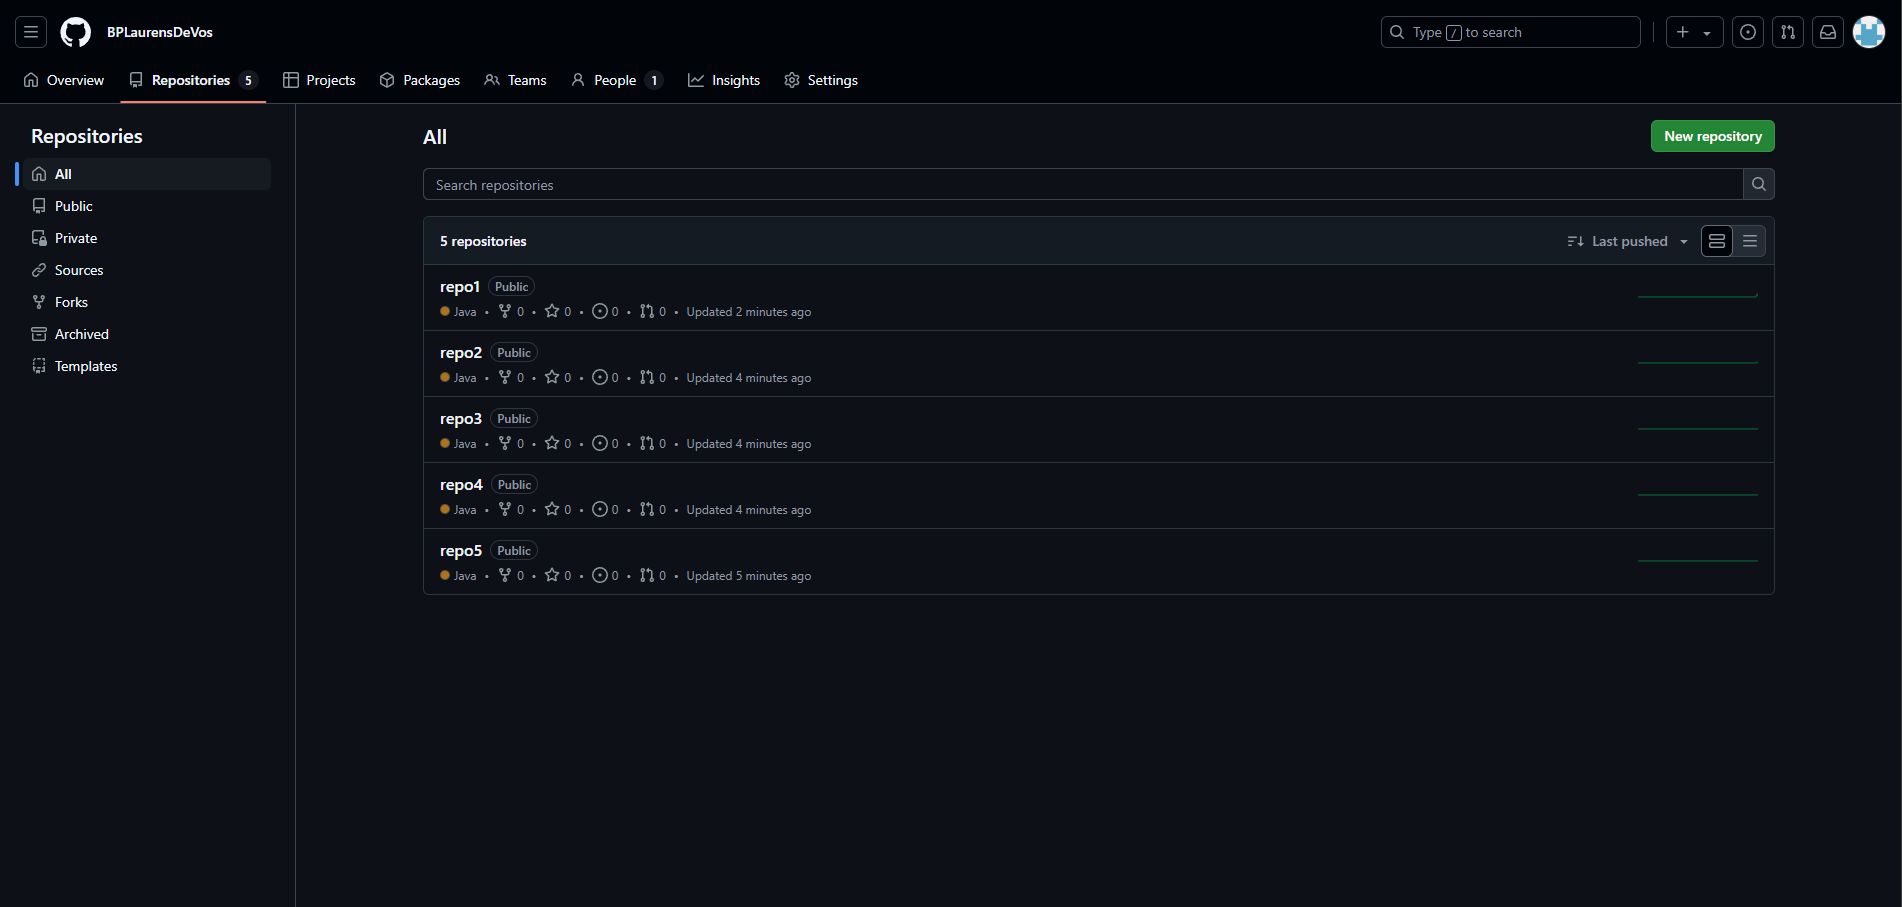
\includegraphics[width=\linewidth]{"C:/Users/laure/Documents/bachelorproef-2024-2025-laurensDeVos/graphics/screenGithubRepo.png"}
    \caption{structuur van alle github repositories}
    \label{fig:repositories}
\end{figure}

\begin{figure}[h!]
    \centering
    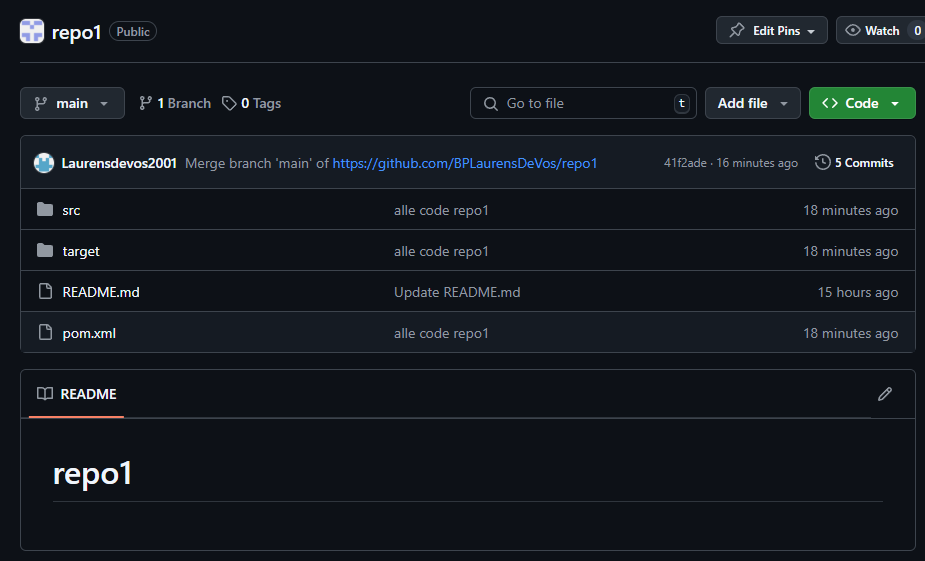
\includegraphics[width=\linewidth]{"C:/Users/laure/Documents/bachelorproef-2024-2025-laurensDeVos/graphics/structuurRepo1.png"}
    \caption{structuur van repo1}
    \label{fig:structuur}
\end{figure}

\ref{fig:repositories}
\ref{fig:structuur}

\subsection{Genereren van de Maven-projecten}
Elk van de vijf repositories is gecreëerd met behulp van de \texttt{maven-archetype-quickstart} template, een standaard template voor Java-projecten in Maven. De volgende commando's zijn gebruikt om een basisproject aan te maken (voor \texttt{Repo1}):

\begin{verbatim}
    mvn archetype:generate "-DgroupId=com.example.repo1" \
    "-DartifactId=repo1" \
    "-DarchetypeArtifactId=maven-archetype-quickstart" \
    "-DinteractiveMode=false"
\end{verbatim}


Het bovenstaande proces is herhaald voor \texttt{Repo2} tot en met \texttt{Repo5}, waarbij de \texttt{groupId} en \texttt{artifactId} telkens zijn aangepast.

\subsection{Afhankelijkheden instellen}
De afhankelijkheden tussen de repositories zijn ingesteld in de \texttt{pom.xml}-bestanden. Zo is \texttt{Repo2} afhankelijk gemaakt van \texttt{Repo1}, terwijl \texttt{Repo3} afhankelijk is van \texttt{Repo2}, enzovoort. Het volgende voorbeeld toont een fragment van de \texttt{pom.xml} van \texttt{Repo2}:

\begin{verbatim}
    <dependencies>
    <dependency>
    <groupId>com.example.repo1</groupId>
    <artifactId>repo1</artifactId>
    <version>1.0-SNAPSHOT</version>
    </dependency>
    </dependencies>
\end{verbatim}

Het configureren van de afhankelijkheden zorgt ervoor dat de build van een repository automatisch de afhankelijkheden downloadt en gebruikt.

\subsection{Toevoegen van dummy code}
Om de functionaliteiten van de repositories te simuleren, is in elke repository eenvoudige Java-code toegevoegd die de afhankelijkheden benut. De codebase is ontworpen om:
\begin{itemize}
    \item De onderlinge afhankelijkheden expliciet te maken.
    \item Te testen of de functionaliteiten correct werken via unit tests.
\end{itemize}

Hieronder volgt een voorbeeld van een simpele klasse in \texttt{Repo1}:

\begin{verbatim}
    package com.example.repo1;
    
    public class Utility {
        public static String getMessage() {
            return "Hello from Repo1!";
        }
    }
\end{verbatim}

Een voorbeeld van een afhankelijkheid in \texttt{Repo2}:

\begin{verbatim}
    package com.example.repo2;
    
    import com.example.repo1.Utility;
    
    public class Service2 {
        public String getServiceMessage() {
            return Utility.getMessage() + " Called by Repo2.";
        }
    }
\end{verbatim}

De volledige broncode is te vinden in de github organisatie \url{https://github.com/BPLaurensDeVos}

\subsection{Unit tests}
In elke repository zijn unit tests toegevoegd om de correctheid van de implementatie te waarborgen. Deze tests zijn geschreven met behulp van JUnit 5, een moderne en uitgebreide testbibliotheek. De volgende code toont een voorbeeld van een unit test in \texttt{Repo2}:

\begin{verbatim}
    package com.example.repo2;
    
    import org.junit.jupiter.api.Test;
    import static org.junit.jupiter.api.Assertions.assertEquals;
    
    public class Service2Test {
        @Test
        public void testGetServiceMessage() {
            Service2 service = new Service2();
            assertEquals("Hello from Repo1! Called by Repo2.", 
            service.getServiceMessage());
        }
    }
\end{verbatim}

De tests worden uitgevoerd met het volgende commando:
\begin{verbatim}
    mvn clean test
\end{verbatim}

\subsection{Lokale installatie en controle}
Na het instellen van de afhankelijkheden en toevoegen van de dummy code zijn de repositories lokaal geïnstalleerd met het volgende commando:
\begin{verbatim}
    mvn clean install
\end{verbatim}

Dit commando genereert de vereiste artefacten (zoals JAR-bestanden) en controleert de correcte werking van de afhankelijkheden.

\begin{figure}[h!]
    \centering
    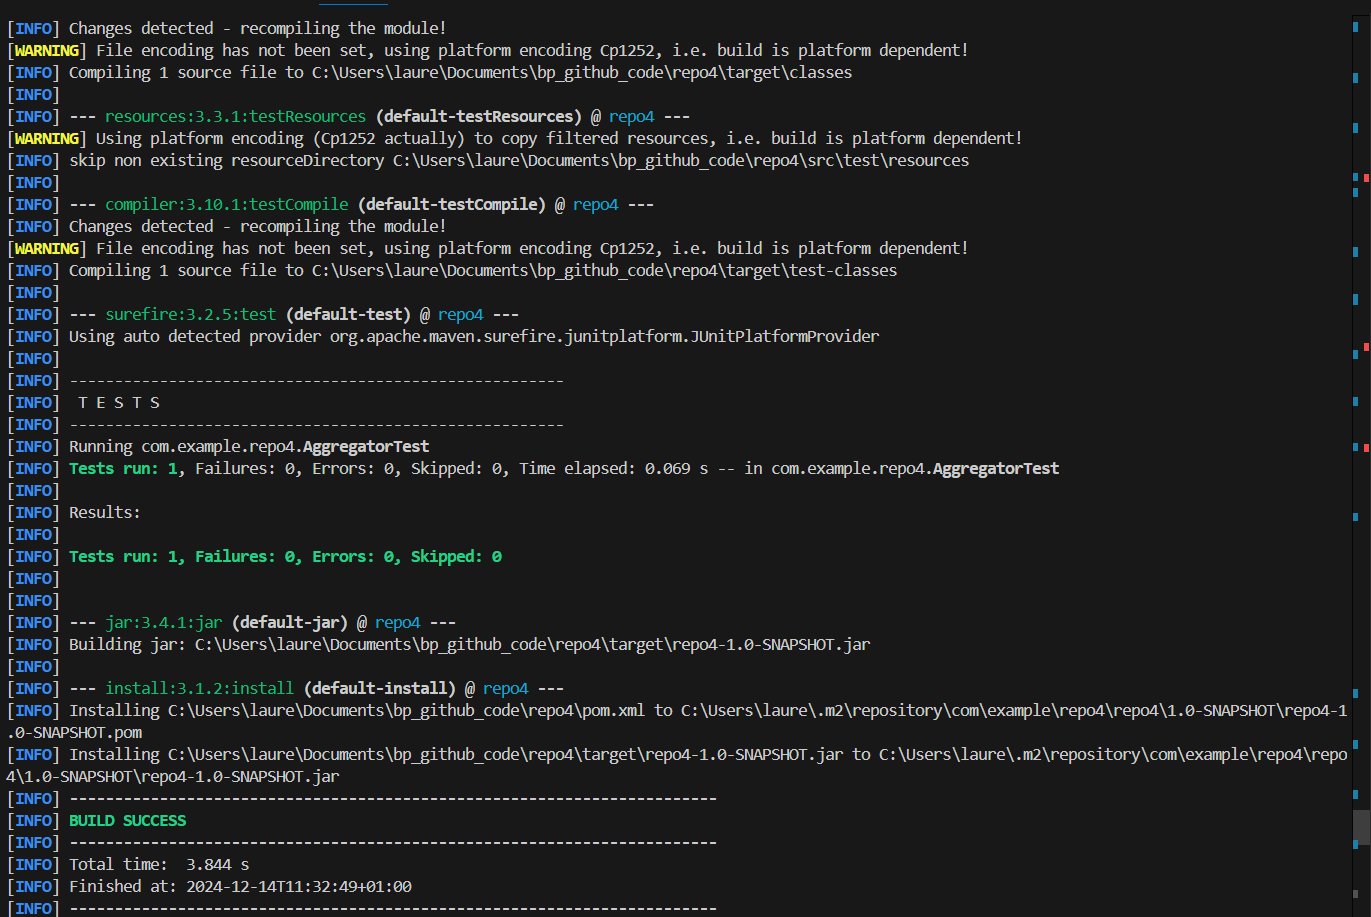
\includegraphics[width=\linewidth]{"C:/Users/laure/Documents/bachelorproef-2024-2025-laurensDeVos/graphics/voorbeeldOutput.png"}
    \caption{De output van 'mvn clean install' in repo4}
    \label{fig:mvncleaninstall}
\end{figure}

De afbeelding \ref{fig:mvncleaninstall} toont de output gegenereerd door vorig commando.


\subsection{GitHub-integratie}
Alle repositories zijn geüpload naar GitHub onder de organisatie \texttt{BPLaurensDeVos}. Een voorbeeld van het pushen van de code naar GitHub:

\begin{verbatim}
    git init
    git remote add origin https://github.com/BPLaurensDeVos/repo1.git
    git add .
    git commit -m "eerste commit repo1"
    git branch -M main
    git push -u origin main --force
\end{verbatim}

\subsection{Conclusie}
Met deze opzet is een solide basis gelegd voor het testen van Jenkins en GitHub Actions. De gekozen structuur en dummy code maken het mogelijk om complexe workflows te simuleren en de tools eerlijk te vergelijken op basis van de gestelde evaluatiecriteria.


\section{Ontwerp en Implementatie van CI/CD-pipelines}

\subsection{Inleiding}
Het opzetten van CI/CD-pipelines in zowel Jenkins als GitHub Actions vormt een cruciaal onderdeel van deze studie. Deze pipelines zijn ontworpen om de workflows van vijf Java-repositories met onderlinge afhankelijkheden te simuleren. Het doel is om de tools te configureren met een identieke structuur en workflow, zodat een eerlijke vergelijking mogelijk is.

De CI/CD-pipelines bestaan uit de volgende stappen:
\begin{itemize}
    \item \textbf{Build}: Het compileren van de Java-code met Maven.
    \item \textbf{Test}: Het uitvoeren van unit tests om de functionaliteit te valideren.
    \item \textbf{Deploy}: Het publiceren van artefacten naar Github Packages.
    \item \text{SonarCloud scan}: Het uitvoeren van code quality checks met SonarCloud.
\end{itemize}

De afhankelijkheden tussen de repositories worden expliciet beheerd, zodat de workflows correct functioneren. In deze sectie worden de implementaties in Jenkins en GitHub Actions apart behandeld.

\subsection{Implementatie van CI/CD met GitHub Actions}

GitHub Actions biedt een native CI/CD-oplossing die naadloos integreert met GitHub. Voor deze Proof-of-Concept werd GitHub Actions gebruikt om pipelines op te zetten voor vijf Java-repositories met onderlinge afhankelijkheden. Elke repository heeft zijn eigen pipeline, waarbij artefacten van andere repositories worden gedownload via GitHub Packages. 

\subsubsection{Doelstellingen van de CI/CD-pipeline}
De GitHub Actions-pipelines zijn ontworpen om:
\begin{itemize}
    \item \textbf{De Java-code te bouwen}: Het compileren van de code in elke repository met behulp van Maven.
    \item \textbf{Unit tests uit te voeren}: JUnit-tests draaien om de functionaliteit van de code te valideren.
    \item \textbf{Artefacten te publiceren}: Gereedgemaakte artefacten (JAR-bestanden) naar GitHub Packages publiceren.
    \item \textbf{Afhankelijkheden te beheren}: Controleren of benodigde artefacten beschikbaar zijn en indien nodig upstream repositories aanroepen.
    \item \textbf{SonarCloud-integratie}: Uitvoeren van code quality checks via SonarCloud.
\end{itemize}

\subsubsection{Voorbereiding van het project} \label{subsec:voorbereidingvanhetproject}

Bij de implementatie van de Proof-of-Concept (PoC) voor het vergelijken van Jenkins en GitHub Actions was een grondige voorbereiding noodzakelijk. Deze voorbereiding omvatte het opzetten van repositories, het configureren van SonarCloud voor kwaliteitsanalyse, en het instellen van de benodigde secrets in GitHub. De stappen in dit proces worden hieronder beschreven.

\begin{enumerate}
    \item \textbf{Aanmaken van repositories}:
    \begin{itemize}
        \item Elk van de vijf repositories (\texttt{Repo1} tot \texttt{Repo5}) werd geconfigureerd in GitHub onder de organisatie \texttt{BPLaurensDeVos}. 
        \item Elke repository bevat:
        \begin{itemize}
            \item Een Maven-project, met een \texttt{pom.xml} die afhankelijkheden en build-configuraties definieert.
            \item Dummy-code om onderlinge afhankelijkheden tussen de repositories te simuleren.
            \item Unit tests geschreven in JUnit 5, die dienen om de functionaliteit van de code te valideren.
        \end{itemize}
    \end{itemize}
    
    \item \textbf{Aanmaken van SonarCloud}:
    SonarCloud werd geïntegreerd om statische code-analyse, kwaliteitsbewaking en beveiligingscontroles uit te voeren. Het proces omvatte:
    \begin{enumerate}
        \item \textbf{Registratie en organisatie-instelling}:
        \begin{itemize}
            \item Een SonarCloud-account werd aangemaakt via \url{https://sonarcloud.io}, gebruikmakend van GitHub-authenticatie.
            \item Een organisatie genaamd \texttt{BPLaurensDeVos} werd opgezet binnen SonarCloud, gekoppeld aan de GitHub-organisatie.
        \end{itemize}
        
        \item \textbf{Projectconfiguratie}:
        \begin{itemize}
            \item Vier van de vijf repositories (Repo2 tot en met Repo5) werden toegevoegd als een project in SonarCloud. 
            \item Voor elk project werd een unieke \texttt{sonar.projectKey} gegenereerd, die wordt gebruikt tijdens de analyse.
        \end{itemize}
        
        \item \textbf{Genereren van een SonarCloud-token}:
        \begin{itemize}
            \item Een token werd aangemaakt in SonarCloud via \texttt{My Account > Security}.
            \item Dit token werd geconfigureerd als een GitHub secret genaamd \texttt{SONAR\_TOKEN} in elk van de vijf repositories.
        \end{itemize}
    \end{enumerate}
    
    \item \textbf{Configureren van GitHub Secrets}:
    Om de CI/CD-pipelines succesvol te laten werken, werden de volgende secrets geconfigureerd in GitHub:
    \begin{itemize}
        \item \texttt{PAT\_TOKEN}: Een Personal Access Token (PAT) werd aangemaakt met de volgende rechten:
        \begin{itemize}
            \item \texttt{read:packages} en \texttt{write:packages} om artefacten te downloaden en uploaden in GitHub Packages.
            \item \texttt{repo} om toegang te krijgen tot de repositories en workflows.
        \end{itemize}
        Het token werd toegevoegd als een GitHub secret met de naam \texttt{PAT\_TOKEN} in elk van de repositories.
        
        \item \texttt{SONAR\_TOKEN}: Een SonarCloud-authenticatietoken werd aangemaakt en geconfigureerd om de SonarCloud-scan te autoriseren. Dit omvatte:
        \begin{itemize}
            \item Het genereren van het token in SonarCloud.
            \item Het toevoegen van het token als een GitHub secret genaamd \texttt{SONAR\_TOKEN} in de organisatie.
        \end{itemize}
    \end{itemize}
\end{enumerate}


In de afbeelding \ref{fig:PATTOKEN} is te zien dat een Personal Acces Token werd aangemaakt in Settings $\rightarrow$ Developer Settings $\rightarrow$ Personal acces tokens $\rightarrow$ Tokens(classic).

\begin{figure}[h!]
    \centering
    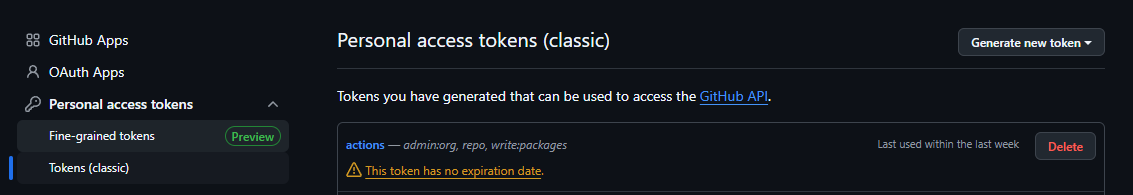
\includegraphics[width=\linewidth]{"C:/Users/laure/Documents/bachelorproef-2024-2025-laurensDeVos/graphics/pat_token.png"}
    \caption{Personal Acces Token.}
    \label{fig:PATTOKEN}
\end{figure}

\begin{figure}[h!]
    \centering
    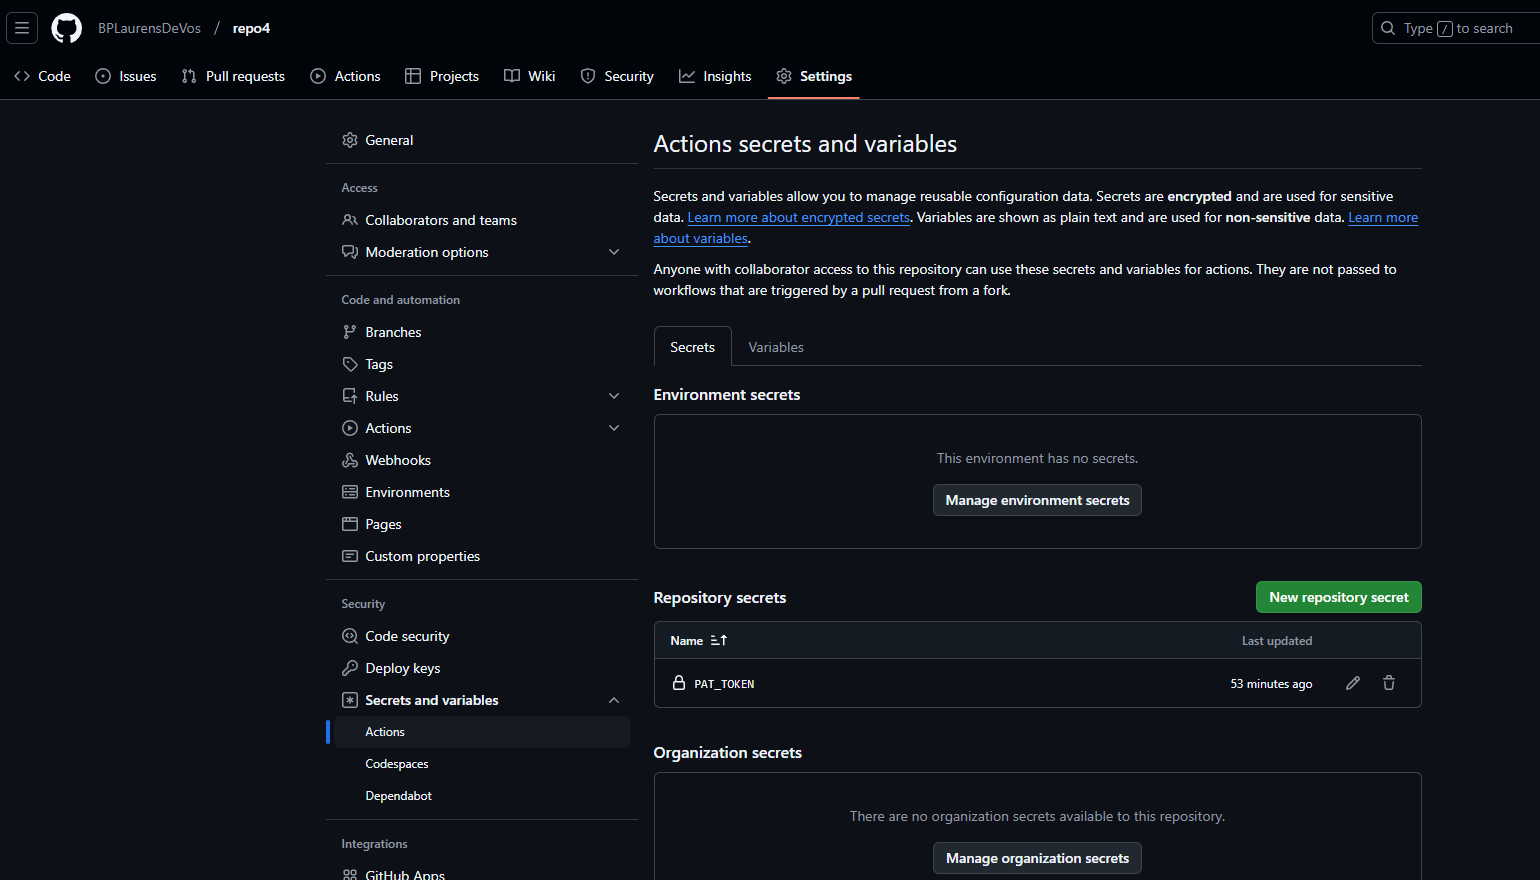
\includegraphics[width=\linewidth]{"C:/Users/laure/Documents/bachelorproef-2024-2025-laurensDeVos/graphics/tokenRepo.png"}
    \caption{Voorbeeld van de token toegevoegd als secret in Repo5.}
    \label{fig:tokenRepo}
\end{figure}

\subsubsection{Workflowconfiguratie in GitHub Actions}

In deze subsubsectie wordt het proces beschreven van het opzetten en configureren van de workflows in GitHub Actions voor de vijf repositories. Elke repository heeft een unieke workflow, gebaseerd op een herbruikbare structuur met specifieke aanpassingen afhankelijk van de afhankelijkheden van de repository.

\paragraph{Algemene structuur van de workflow}
De workflows in GitHub Actions worden gedefinieerd in YAML-bestanden onder de map \texttt{.github/workflows/}. Het basisworkflowbestand bestaat uit de volgende secties:
\begin{enumerate}
    \item \textbf{Triggers}: Bepaalt wanneer de workflow wordt uitgevoerd.
    \item \textbf{Jobs}: Beschrijft de specifieke taken die in de workflow moeten worden uitgevoerd.
    \item \textbf{Environment Configuration}: Voorzien van secrets zoals \texttt{PAT\_TOKEN} en configuratie van Maven.
\end{enumerate}

\paragraph{Triggers}
De workflows worden uitgevoerd bij:
\begin{itemize}
    \item Een \texttt{push} naar de \texttt{main}-branch.
    \item Een \texttt{repository\_dispatch}-event, gebruikt om downstream workflows te activeren.
\end{itemize}

\textbf{Codevoorbeeld:}

\begin{verbatim}
    on:
      push:
        branches:
          - main
      repository_dispatch:
        types:
          - build-artifact
\end{verbatim}

\begin{figure}[h!]
    \centering
    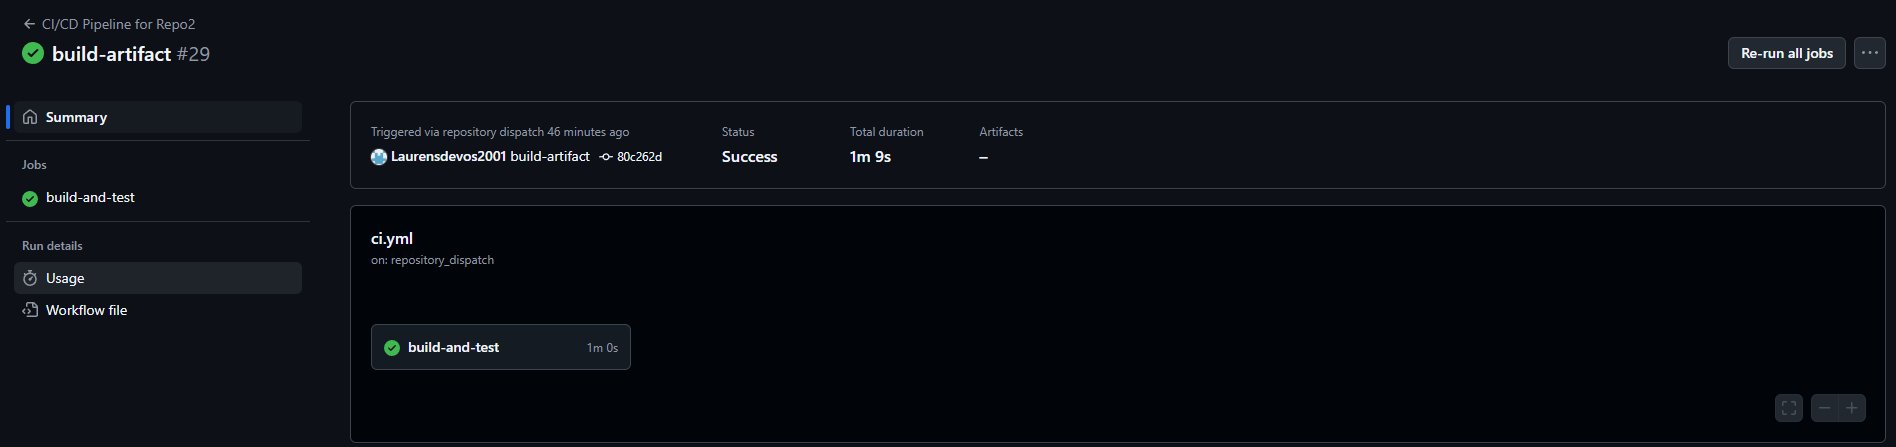
\includegraphics[width=\linewidth]{"C:/Users/laure/Documents/bachelorproef-2024-2025-laurensDeVos/graphics/uitgevoerdeWorkflow.png"}
    \caption{een workflow (repo1) uitgevoerd door \texttt{repository\_dispatch}.}
    \label{fig:uitgevoerdeWorkflow}
\end{figure}

\paragraph{Gedetailleerde beschrijving van de jobs}
De jobs in elke workflow volgen een herbruikbaar patroon, met unieke stappen voor afhankelijkheden. Hieronder volgt een voorbeeld van de workflow voor \texttt{Repo1}.

\subparagraph{Stap 1: Checkout van de repository}
Met behulp van de \texttt{actions/checkout@v3}-actie wordt de meest recente code opgehaald uit de GitHub-repository.

\begin{verbatim}
    - name: Checkout Repository
      uses: actions/checkout@v3
\end{verbatim}

\begin{figure}[h!]
    \centering
    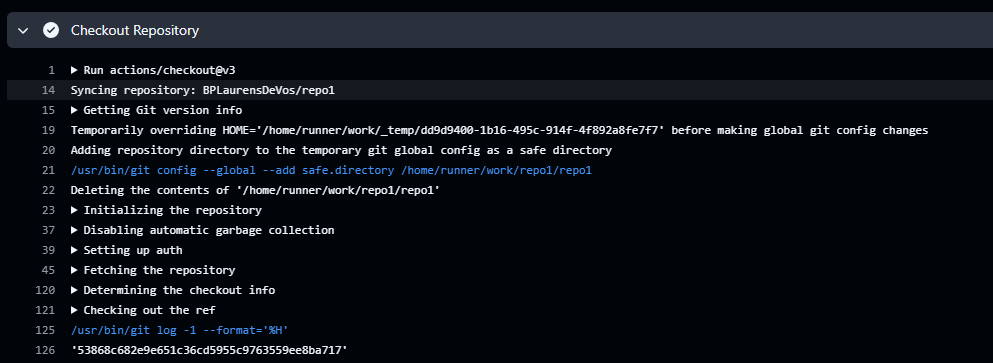
\includegraphics[width=\linewidth]{"C:/Users/laure/Documents/bachelorproef-2024-2025-laurensDeVos/graphics/checkout1.png"}
    \caption{Succesvolle uitvoer van de Checkout Repository job}
    \label{fig:check1}
\end{figure}

\subparagraph{Stap 2: Configureren van JDK 17}
De actie \texttt{actions/setup-java@v3} configureert Java 17, een vereiste voor het Maven-buildproces.

\begin{verbatim}
    - name: Set up JDK 17
      uses: actions/setup-java@v3
      with:
        java-version: 17
        distribution: 'temurin'
\end{verbatim}

\begin{figure}[h!]
    \centering
    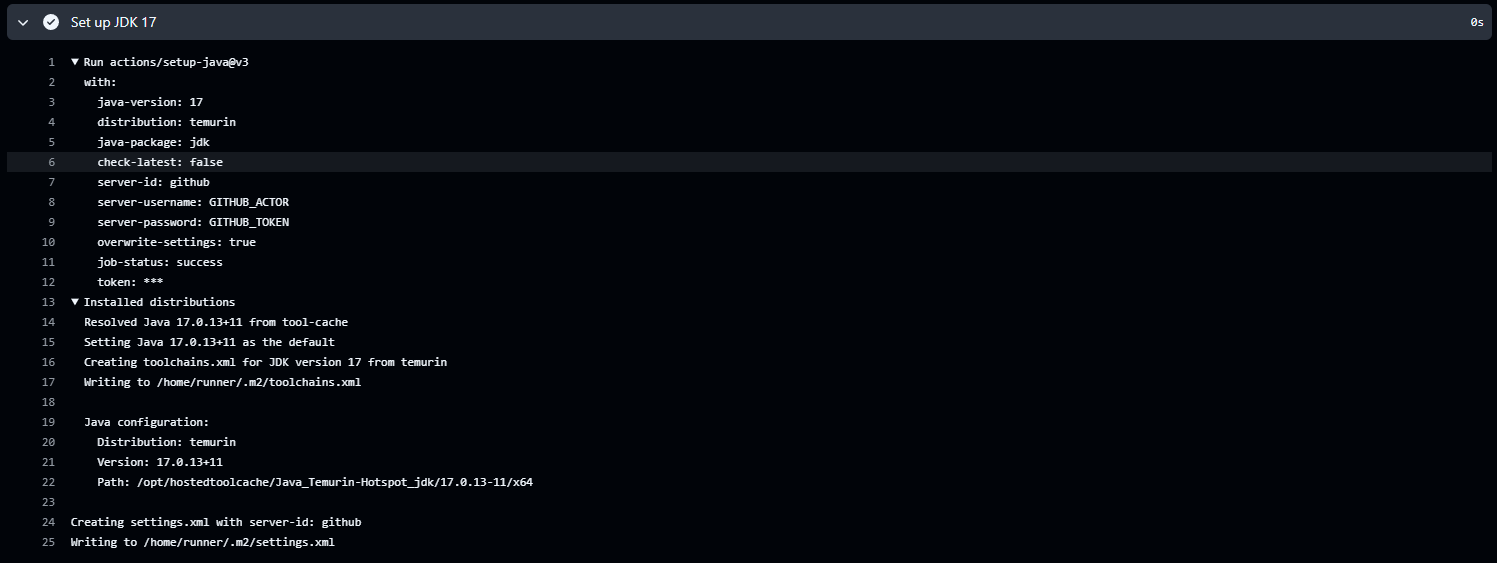
\includegraphics[width=\linewidth]{"C:/Users/laure/Documents/bachelorproef-2024-2025-laurensDeVos/graphics/java1.png"}
    \caption{Succesvolle uitvoer van de Set up JDK 17 Repository job}
\end{figure}

\subparagraph{Stap 3: Build en Test}
De code wordt gebouwd en de tests worden uitgevoerd met behulp van Maven-commando's. Dit valideert de functionaliteit van de code.

\begin{verbatim}
    - name: Build and Test
      run: mvn clean package
\end{verbatim}

\begin{figure}[h!]
    \centering
    \includegraphics[width=\linewidth]{"C:/Users/laure/Documents/bachelorproef-2024-2025-laurensDeVos/graphics/Buildpackage1.png"}
    \caption{Build succes toont aan dat de de applicatie is opgebouwd en getest}
\end{figure}


\subparagraph{Stap 4: Publiceren naar GitHub Packages}
Artefacten (zoals JAR-bestanden) worden gepubliceerd naar GitHub Packages met behulp van het \texttt{mvn deploy}-commando. 

\begin{verbatim}
    - name: Publish to GitHub Packages
      run: mvn deploy
      env:
        GITHUB_ACTOR: ${{ github.actor }}
        GITHUB_TOKEN: ${{ secrets.PAT_TOKEN }}
\end{verbatim}

\begin{figure}[h!]
    \centering
    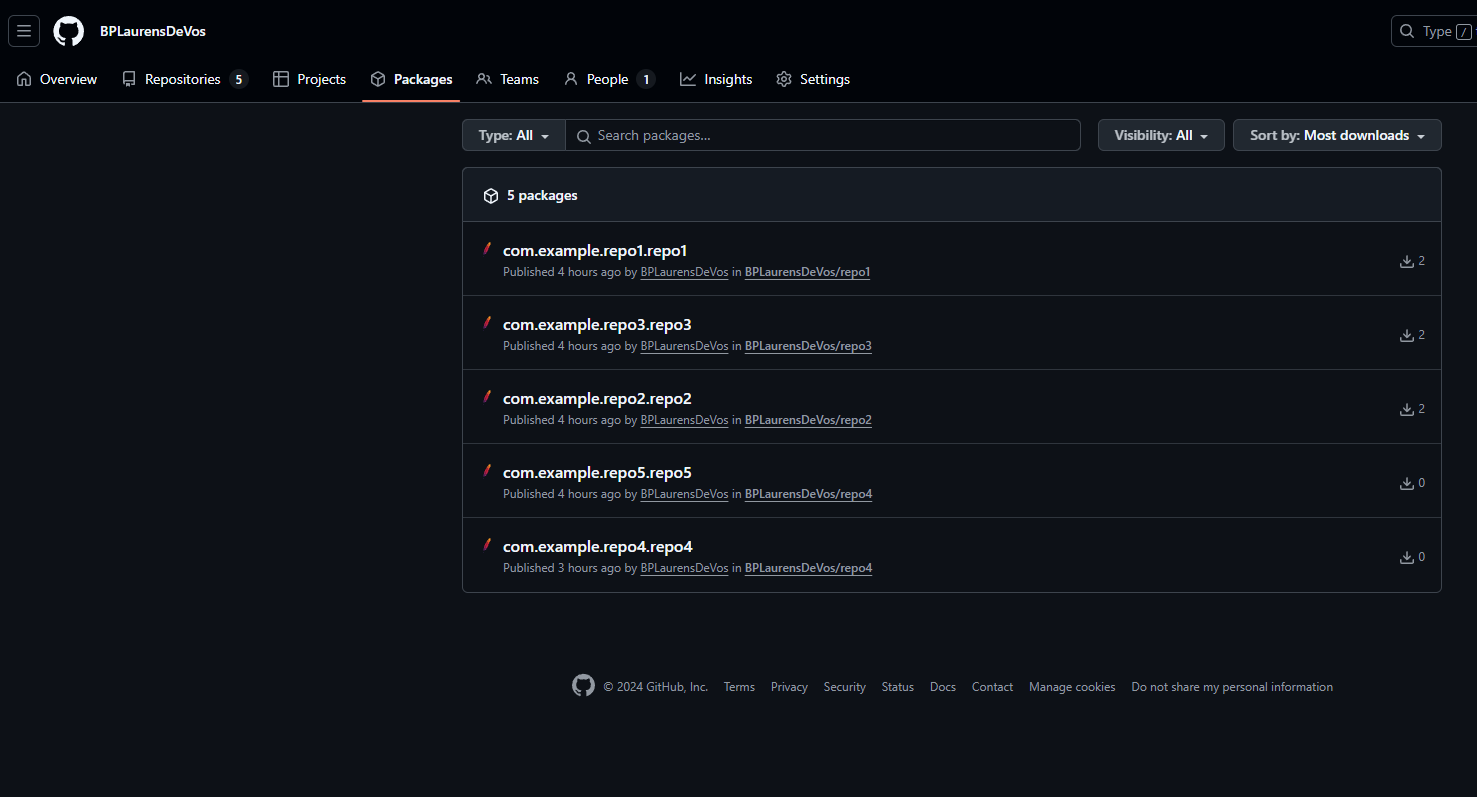
\includegraphics[width=\linewidth]{"C:/Users/laure/Documents/bachelorproef-2024-2025-laurensDeVos/graphics/packages.png"}
    \caption{Alle artifacts zijn te vinden in de GitHub organisatie (BPLaurensDeVos) onder $\rightarrow$ Packages}
\end{figure}

\paragraph{Complete workflow voor Repo1}
Hieronder volgt het volledige YAML-bestand van de workflow voor \texttt{Repo1}:

\begin{verbatim}
    name: CI/CD Pipeline for Repo1
    
    on:
      push:
        branches:
          - main
      repository_dispatch:
        types:
          - build-artifact
    
    jobs:
      build-and-test:
        runs-on: ubuntu-latest
        steps:
          - name: Checkout Repository
            uses: actions/checkout@v3
    
          - name: Set up JDK 17
            uses: actions/setup-java@v3
            with:
              java-version: 17
              distribution: 'temurin'
    
          - name: Build and Test
            run: mvn clean package
    
          - name: Publish to GitHub Packages
            run: mvn deploy
            env:
              GITHUB_ACTOR: ${{ github.actor }}
              GITHUB_TOKEN: ${{ secrets.PAT_TOKEN }}
\end{verbatim}

Voor een visueel overzicht van een succesvolle uitvoering van de workflow in \texttt{Repo1}, zie Appendix~\ref{fig:workflow-repo1}.

\paragraph{Specifieke workflows voor downstream repositories}
Repositories zoals \texttt{Repo2} tot \texttt{Repo5} vereisen aanvullende configuraties vanwege hun afhankelijkheden. Voor deze repositories moet eerst worden gecontroleerd of de artefacten van de bijbehorende afhankelijkheden beschikbaar zijn in de GitHub Package Registry. Indien de benodigde artefacten niet beschikbaar zijn, wordt de workflow van de afhankelijke repository gestart via een \texttt{repository\_dispatch}-event om de artefacten alsnog te genereren.

\subparagraph{1. Controleren van artefactbeschikbaarheid}
Om ervoor te zorgen dat de build van een repository correct kan worden uitgevoerd, moeten alle benodigde artefacten van afhankelijkheden beschikbaar zijn in GitHub Packages. Dit wordt gedaan door een HTTP-verzoek uit te voeren naar het specifieke artefact in de package registry van GitHub. De \texttt{curl}-tool wordt gebruikt om een statuscode te verkrijgen die aangeeft of het artefact beschikbaar is.

\begin{itemize} 
    \item Statuscode 200: Het artefact is beschikbaar, wat betekent dat de afhankelijkheid succesvol kan worden gedownload en gebruikt. \item Andere statuscodes: Het artefact is niet beschikbaar, wat betekent dat de workflow van de upstream repository moet worden gestart om het artefact te genereren en te publiceren. 
\end{itemize}

\textbf{Deel van de code in Repo2}:

\begin{verbatim}
    - name: Check Repo1 Artifact Availability
      run: |
            STATUS_CODE=$(curl -L -u ${{ github.actor }}:${{ secrets.PAT_TOKEN }} \
                -s \
                -o /dev/null \
                -w "%{http_code}" \
                https://maven.pkg.github.com/BPLaurensDeVos/repo1/com/example/repo1/repo1/1.0/repo1-1.0.jar)
        echo "Artifact Status Code: $STATUS_CODE"
        echo "repo1_status_code=$STATUS_CODE" >> $GITHUB_ENV
\end{verbatim}

\begin{figure}[h!]
    \centering
    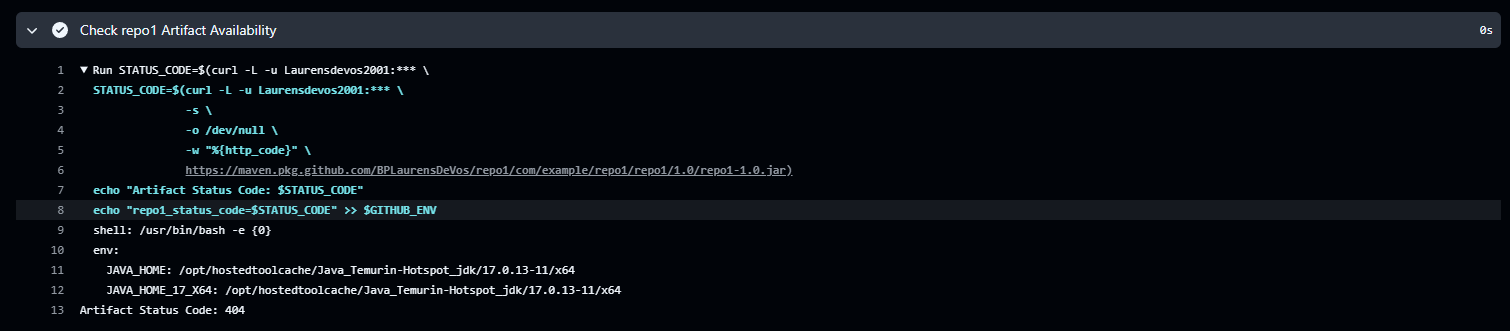
\includegraphics[width=\linewidth]{"C:/Users/laure/Documents/bachelorproef-2024-2025-laurensDeVos/graphics/status404.png"}
    \caption{Voorbeeld uit repo2 waar het artefact niet gevonden wordt en Status Code 404 wordt gegeven. }
\end{figure}

\begin{figure}[h!]
    \centering
    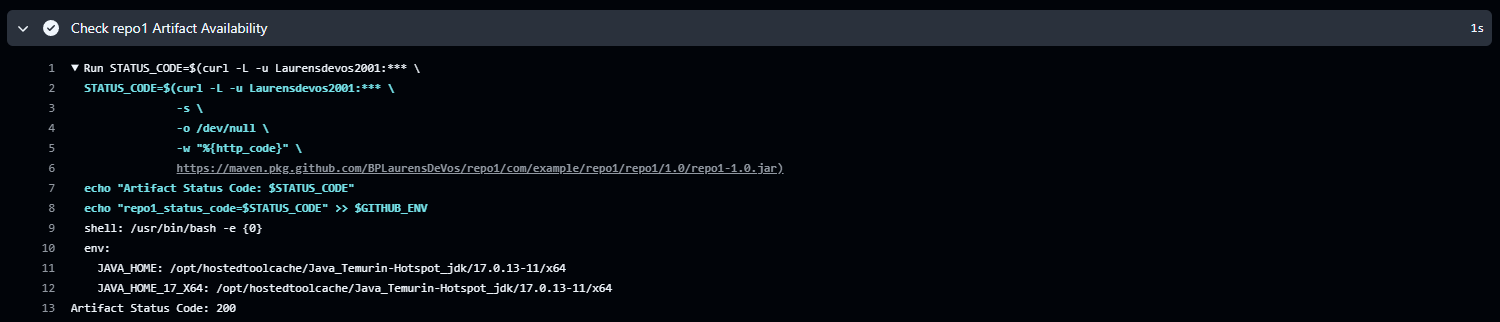
\includegraphics[width=\linewidth]{"C:/Users/laure/Documents/bachelorproef-2024-2025-laurensDeVos/graphics/status200.png"}
    \caption{Voorbeeld uit repo2 waar het artefact wel gevonden wordt en Status Code 200 wordt gegeven. }
\end{figure}

\subparagraph{2. Triggeren van upstream workflows}
Wanneer een afhankelijk artefact niet beschikbaar is in GitHub Packages, moet de workflow van de upstream repository worden gestart. Dit gebeurt door een \texttt{repository\_dispatch}-event te versturen met behulp van de \texttt{curl}-tool. Dit mechanisme zorgt ervoor dat downstream repositories niet vastlopen door ontbrekende afhankelijkheden, maar in plaats daarvan de benodigde artefacten actief opvragen.

\textbf{Deel van de code in Repo2}:

\begin{verbatim}
    - name: Trigger Repo1 if Artifact is Missing
      if: env.repo1_status_code != '200'
      run: |
        curl -X POST \
        -H "Accept: application/vnd.github.v3+json" \
        -H "Authorization: token ${{ secrets.PAT_TOKEN }}" \
           https://api.github.com/repos/BPLaurensDeVos/repo1/dispatches \
        -d '{"event_type":"build-artifact"}'
\end{verbatim}

\begin{figure}[h!]
    \centering
    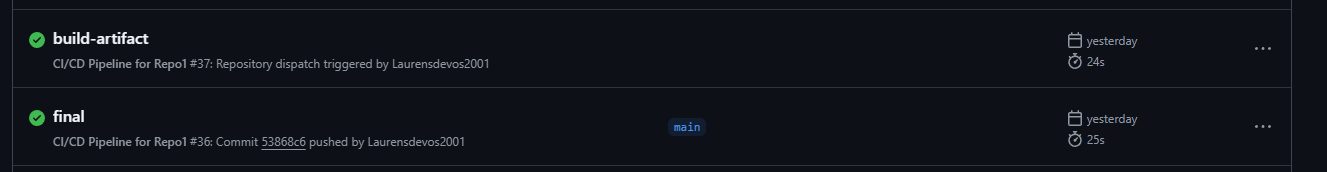
\includegraphics[width=\linewidth]{"C:/Users/laure/Documents/bachelorproef-2024-2025-laurensDeVos/graphics/trigger1.png"}
    \caption{Overzicht van twee workflow-runs: de eerste is gestart door een \texttt{repository\_dispatch}-event met de \texttt{build-artifact}-trigger, terwijl de tweede is gestart door een commit naar de \texttt{main}-branch.}
\end{figure}

\subparagraph{3. Wachten tot het artefact gepubliceerd is}
Nadat de workflow van een upstream repository is geactiveerd, is het noodzakelijk om te wachten totdat het benodigde artefact beschikbaar is in GitHub Packages. Dit voorkomt dat de downstream workflow mislukt vanwege ontbrekende afhankelijkheden. De wachttijd wordt iteratief verhoogd bij de repositories aangezien repo5 mogelijks moet wachten op alle voorgaande repositories en repo2 enkel op repo1.

\textbf{Waarom wachten?}

\begin{itemize} 
    \item Een \texttt{repository\_dispatch}-event start de workflow in een upstream repository, maar het bouwen en publiceren van een artefact kost tijd. 
    \item Zonder een wachtmechanisme zou de downstream workflow direct doorgaan, wat leidt tot fouten als het artefact nog niet beschikbaar is. 
\end{itemize}

\textbf{Voorbeeld uit de workflow van Repo2}:

\begin{verbatim}
      - name: Wait for Repo1 Artifact to be Published
        if: env.repo1_status_code != '200'
        run: |
            echo "Waiting for Repo1 artifact to be published..."
            sleep 30
\end{verbatim}

\textbf{Voorbeeld uit de workflow van Repo5}:

\begin{verbatim}
    - name: Wait for Repo1 Artifact to be Published
    if: env.repo1_status_code != '200'
    run: |
        echo "Waiting for Repo1 artifact to be published..."
        sleep 180
\end{verbatim}

\subparagraph{4. Opnieuw controleren van artefactbeschikbaarheid}
Nadat de workflow van een upstream repository is uitgevoerd, wordt gecontroleerd of het artefact nu beschikbaar is in GitHub Packages. Deze tweede controle bepaalt of de workflow kan doorgaan of moet worden afgebroken wegens ontbrekende afhankelijkheden.

\textbf{Belang van deze stap}:

\begin{itemize} 
    \item Zorgt ervoor dat de workflow alleen doorgaat wanneer alle benodigde artefacten beschikbaar zijn. 
    \item Minimaliseert het risico op fouten verderop in het proces door afhankelijkheden tijdig te valideren. 
\end{itemize}

\textbf{Voorbeeld uit de workflow van Repo2}:

\begin{verbatim}
      - name: Recheck Artifact Availability
        if: env.repo1_status_code != '200'
        id: recheck-artifact
        run: |
            STATUS_CODE=$(curl -L -u ${{ github.actor }}:${{        secrets.PAT_TOKEN }} \
                -s \
                -o /dev/null \
                -w "%{http_code}" \
                https://maven.pkg.github.com/BPLaurensDeVos/repo1/com/example/repo1/repo1/1.0/repo1-1.0.jar)
            echo "Rechecked Artifact Status Code: $STATUS_CODE"
            echo "repo1_recheck_status_code=$STATUS_CODE" >> $GITHUB_ENV
\end{verbatim}

\subparagraph{5. Falen van de workflow}
Als na de tweede controle blijkt dat het benodigde artefact nog steeds niet beschikbaar is in GitHub Packages, wordt de workflow bewust gestopt. Dit voorkomt dat de pipeline verdergaat zonder de vereiste afhankelijkheden, wat later tot build- of runtime-fouten zou kunnen leiden.

\textbf{Voorbeeld uit de workflow van Repo2}:

\begin{verbatim}
      - name: Fail Workflow if Artifact Still Missing
        if: env.repo1_status_code != '200' && env.repo1_recheck_status_code != '200'
        run: |
            echo "Artifact still missing after waiting. Failing workflow..."
            exit 1
\end{verbatim}

\subparagraph{6. Configureren van Maven}
Om ervoor te zorgen dat Maven geauthenticeerd kan communiceren met GitHub Packages, wordt in de workflow dynamisch een aangepaste \texttt{settings.xml}-configuratie gegenereerd. Deze configuratie bevat de authenticatiegegevens van de gebruiker en zorgt ervoor dat Maven toegang heeft tot de package repositories.

\begin{verbatim}
      - name: Configure Maven to Use GitHub Packages
        if: env.repo1_status_code == '200' ||                          env.repo1_recheck_status_code == '200'
        run: |
            mkdir -p ~/.m2
            echo "<settings xmlns='http://maven.apache.org/SETTINGS/1.0.0'
                xmlns:xsi='http://www.w3.org/2001/XMLSchema-instance'
                xsi:schemaLocation='http://maven.apache.org/SETTINGS/1.0.0 https://maven.apache.org/xsd/settings-1.0.0.xsd'>
                <servers>
                    <server>
                        <id>github</id>
                        <username>${{ github.actor }}</username>
                        <password>${{ secrets.PAT_TOKEN }}</password>
                    </server>
                </servers>
              </settings>" > ~/.m2/settings.xml
            cat ~/.m2/settings.xml
\end{verbatim}

Bij \texttt{Repo5} is de configuratie complexer omdat authenticatie vereist is om artefacten van andere repositories te kunnen ophalen. De juiste \texttt{id}'s voor deze repositories worden gespecificeerd in de \texttt{pom.xml}-configuratie van \texttt{Repo5}. De code in de workflow Repo5 is te zien in afbeelding \ref{fig:packages5}.

\begin{figure}[h!]
    \centering
    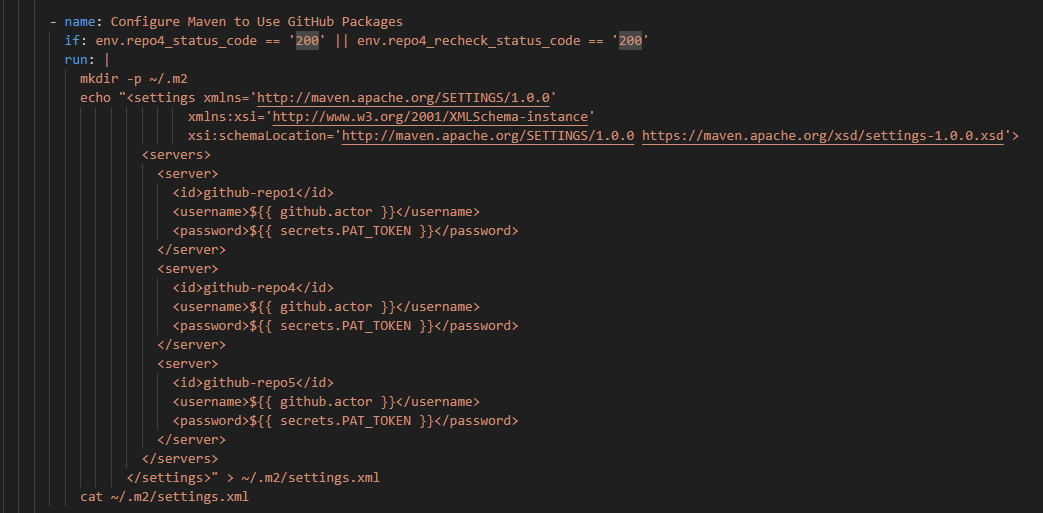
\includegraphics[width=\linewidth]{"C:/Users/laure/Documents/bachelorproef-2024-2025-laurensDeVos/graphics/packages5.png"}
    \caption{pom.xml van repo5.}
    \label{fig:packages5}
\end{figure}

\subparagraph{7. SonarCloud code quality scan}
Om de kwaliteit van de code te waarborgen en beveiligingsproblemen vroegtijdig te detecteren, wordt een statische code-analyse uitgevoerd met behulp van SonarCloud. Deze stap zorgt ervoor dat de repository voldoet aan vooraf gedefinieerde kwaliteitsstandaarden en maakt eventuele technische schulden of kwetsbaarheden inzichtelijk.

\textbf{Belang van deze stap}:
\begin{itemize}
    \item Voorkomt dat slechte codekwaliteit wordt geïntegreerd in de repository.
    \item Identificeert beveiligingslekken en mogelijke bugs.
    \item Bewaakt de onderhoudbaarheid van de codebase door duplicatie en complexe code te minimaliseren.
\end{itemize}

\textbf{Configuratie in de workflow van Repo2}:
De SonarCloud-scan wordt uitgevoerd met behulp van Maven Sonar Plugin. Deze actie gebruikt de eerder ingestelde \texttt{SONAR\_TOKEN} voor authenticatie en maakt gebruik van de instellingen die in de \texttt{pom.xml} zijn opgenomen.

\begin{verbatim}
    - name: SonarCloud Scan
      if: env.repo1_status_code == '200' || env.repo1_recheck_status_code == '200'
      env:
        SONAR_TOKEN: ${{ secrets.SONAR_TOKEN }}
      run: |
        mvn sonar:sonar -Dsonar.login=${{ secrets.SONAR_TOKEN }}
\end{verbatim}

\subsubsection{Configuratie van de \texttt{pom.xml}}
Naast de \texttt{settings.xml} speelt de \texttt{pom.xml} een centrale rol in de configuratie van de Maven-builds en afhankelijkheden. Voor elk van de repositories bevat de \texttt{pom.xml} de volgende onderdelen:

\paragraph{Afhankelijkheden}
De afhankelijkheden van andere repositories worden gedefinieerd in de sectie \texttt{<dependencies>}. Bijvoorbeeld:

\texttt{Repo2}, dat afhankelijk is van \texttt{Repo1}:
\begin{verbatim}
    <dependencies>
      <dependency>
        <groupId>com.example.repo1</groupId>
        <artifactId>repo1</artifactId>
        <version>1.0</version>
      </dependency>
    </dependencies>
\end{verbatim}

\begin{itemize}
    \item \texttt{<groupId>} en \texttt{<artifactId>} verwijzen naar de unieke identificatie van de artefacten.
    \item \texttt{<version>} specificeert de gewenste versie van het artefact.
\end{itemize}

\paragraph{Repositories}
Om artefacten uit GitHub Packages op te halen, worden de relevante repositories gedefinieerd in de \texttt{<repositories>}-sectie:

Voorbeeldconfiguratie:
\begin{verbatim}
    <repositories>
      <repository>
        <id>github</id>
        <url>https://maven.pkg.github.com/BPLaurensDeVos/repo1</url>
      </repository>
    </repositories>
\end{verbatim}

\paragraph{DistributionManagement} 
De \texttt{<distributionManagement>}-sectie in de \texttt{pom.xml} specificeert de locatie waar het artefact van de repository moet worden gepubliceerd. Dit is vooral belangrijk voor het correct opslaan van artefacten in GitHub Packages.

Voorbeeldconfiguratie in Repo2:
\begin{verbatim} 
    <distributionManagement>
      <repository> 
        <id>github</id> <url>https://maven.pkg.github.com/BPLaurensDeVos/repo2</url>
      </repository> </distributionManagement> 
    </distributionManagement>
\end{verbatim}

\begin{itemize} 
    \item \texttt{<id>} moet overeenkomen met de configuratie in de \texttt{settings.xml} om correcte authenticatie te garanderen.
    \item \texttt{<url>} verwijst naar de locatie in GitHub Packages waar het artefact moet worden opgeslagen. 
\end{itemize}

Deze configuratie zorgt ervoor dat artefacten na het buildproces automatisch naar de juiste locatie in GitHub Packages worden gepubliceerd, zodat ze beschikbaar zijn voor downstream repositories.

\paragraph{Build-configuratie}
Het buildproces wordt aangepast met behulp van plugins, zoals de Maven Compiler Plugin en de SonarCloud Maven Plugin:

\begin{verbatim}
    <build>
      <plugins>
        <plugin>
            <groupId>org.apache.maven.plugins</groupId>
            <artifactId>maven-compiler-plugin</artifactId>
            <version>3.10.1</version>
            <configuration>
              <source>17</source>
              <target>17</target>
            </configuration>
        </plugin>
        <plugin>
          <groupId>org.sonarsource.scanner.maven</groupId>
          <artifactId>sonar-maven-plugin</artifactId>
          <version>3.9.1.2184</version>
        </plugin>
      </plugins>
    </build>
\end{verbatim}

\paragraph{Properties}
De \texttt{<properties>}-sectie bevat configuraties voor zowel de Maven Compiler Plugin als de SonarCloud integratie. Deze instellingen zorgen voor consistentie in het buildproces en een correcte verbinding met SonarCloud:

\begin{verbatim}
    <properties>
      <maven.compiler.source>17</maven.compiler.source>
      <maven.compiler.target>17</maven.compiler.target>
      <sonar.projectKey>BPLaurensDeVos_repo2</sonar.projectKey>
      <sonar.organization>bplaurensdevos</sonar.organization>
      <sonar.host.url>https://sonarcloud.io</sonar.host.url>
    </properties>
\end{verbatim}

De Java-compiler gebruikt versie 17 voor zowel broncode als doelcode, terwijl SonarCloud wordt geconfigureerd met een unieke projectkey, organisatie en host-URL.

\paragraph{Relatie tussen \texttt{settings.xml} en \texttt{pom.xml}}
De \texttt{settings.xml} zorgt voor de authenticatie en maakt toegang tot de repositories mogelijk, terwijl de \texttt{pom.xml} de structuur, afhankelijkheden en build-definities van het project specificeert. Samen vormen deze bestanden de kern van de Maven-configuratie.


\subsection{Implementatie van CI/CD met Jenkins}

\subsubsection{Inleiding}

Jenkins is een open-source automation server die wordt gebruikt om softwareontwikkeling te versnellen door Continuous Integration en Continuous Deployment (CI/CD)-processen te automatiseren. Het biedt een uitgebreide set aan functionaliteiten via plug-ins en ondersteunt een breed scala aan technologieën, waaronder Maven, SonarQube en Docker.

In deze Proof-of-Concept (PoC) wordt Jenkins geëvalueerd om te bepalen hoe goed het aansluit bij de behoeften van DocShifter in termen van prestaties, beveiliging en integratie met bestaande systemen. Jenkins wordt vergeleken met GitHub Actions, waarbij beide tools worden gebruikt om identieke workflows uit te voeren. Het doel is om een eerlijk en grondig inzicht te krijgen in de sterke en zwakke punten van Jenkins binnen de context van deze simulatie.

\subsubsection{Doelstellingen van de CI/CD-pipeline in Jenkins}

De Jenkins CI/CD-pipelines hebben dezelfde doelstellingen als die in GitHub Actions:
\begin{itemize}
    \item \textbf{Build}: Het compileren van de Java-code met Maven.
    \item \textbf{Test}: Het uitvoeren van unit tests geschreven in JUnit 5.
    \item \textbf{Deploy}: Het publiceren van artefacten naar GitHub Packages.
    \item \textbf{Afhankelijkheden beheren}: Upstream repositories triggeren indien hun artefacten ontbreken.
    \item \textbf{SonarCloud-integratie}: Codekwaliteit controleren en technische schulden identificeren.
\end{itemize}

\subsubsection{Installatie en Configuratie van Jenkins}
\subsubsection{Installatie van Jenkins}

Jenkins is lokaal geïnstalleerd in een Docker-container om een flexibele en reproduceerbare testomgeving te bieden. De installatie werd uitgevoerd met de volgende stappen:

\begin{enumerate}
    \item \textbf{Installeren van Docker Desktop}:
    Docker Desktop werd geïnstalleerd op een Windows-machine. Dit biedt een gemakkelijke manier om Docker-containers te beheren en te starten.
    \item \textbf{Pullen van de Jenkins Docker Image}:
    Het officiële Jenkins Docker-image werd gedownload met het volgende commando:
    \begin{verbatim}
        docker pull jenkins/jenkins:lts
    \end{verbatim}
    \item \textbf{Starten van de Jenkins-container}:
    De container werd gestart met het volgende commando:
    \begin{verbatim}
        docker run -d --name jenkins -p 8080:8080 -p 50000:50000 \
        -v jenkins_home:/var/jenkins_home jenkins/jenkins:lts
    \end{verbatim}
    \item \textbf{Toegang tot de Jenkins webinterface}:
    Na het starten van de container werd Jenkins toegankelijk via \url{http://localhost:8080}.
    \item \textbf{Initialisatie van Jenkins}:
    Tijdens de eerste keer opstarten genereert Jenkins een initiële admin-wachtwoord. Dit wachtwoord werd opgehaald met het volgende commando:
    \begin{verbatim}
        docker exec jenkins cat /var/jenkins_home/secrets/initialAdminPassword
    \end{verbatim}
    \item \textbf{Installeren van plug-ins}:
    Tijdens de eerste configuratie werden de aanbevolen plug-ins automatisch geïnstalleerd. Deze omvatten onder andere:
    \begin{itemize}
        \item \texttt{Pipeline}.
        \item \texttt{GitHub}.
    \end{itemize}
    Na deze automatische installatie werden de volgende aanvullende plug-ins handmatig geïnstalleerd:
    \begin{itemize}
        \item \texttt{Maven Integration} (voor het configureren van Maven-builds).
        \item \texttt{SonarQube Scanner for Jenkins} (voor integratie met SonarCloud).
    \end{itemize}
\end{enumerate}

\begin{figure}[h!]
    \centering
    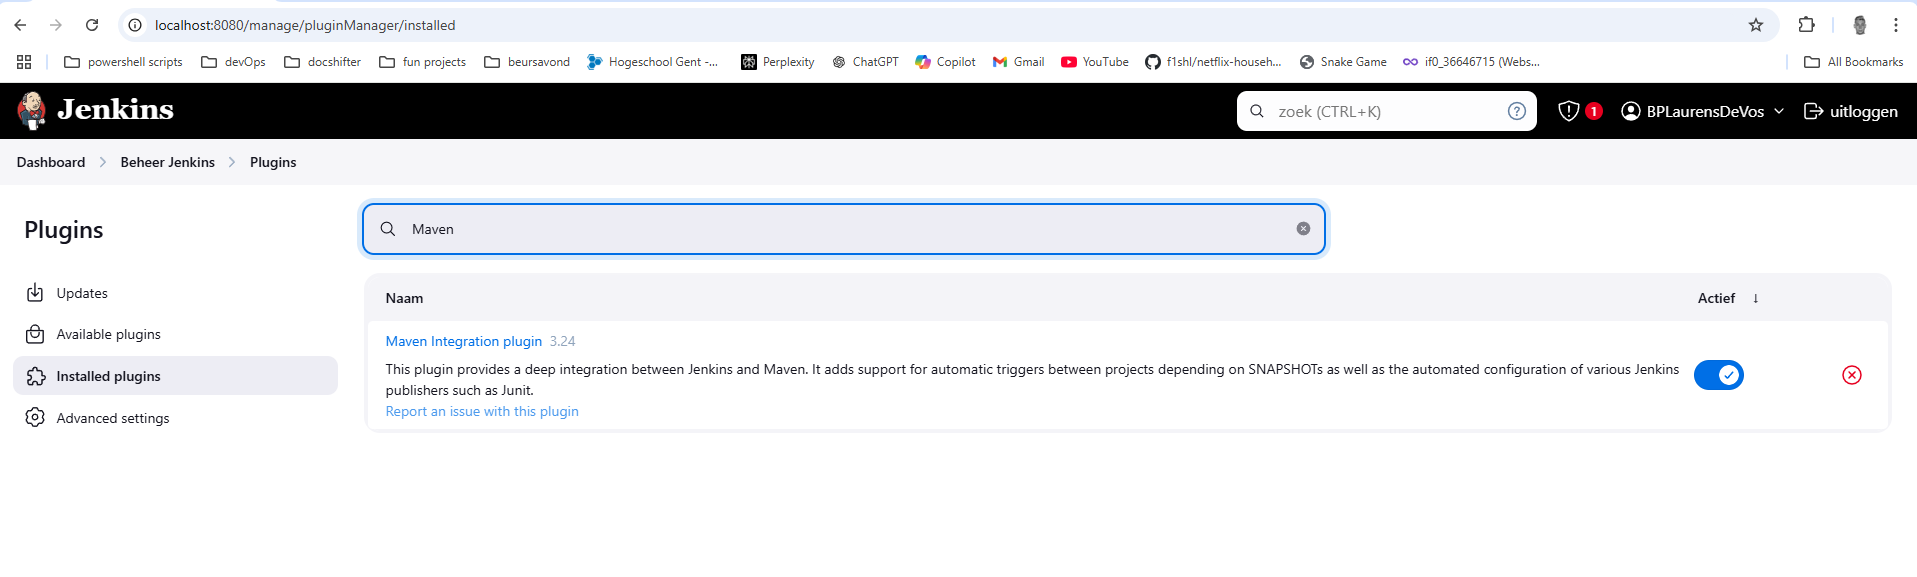
\includegraphics[width=\linewidth]{"C:/Users/laure/Documents/bachelorproef-2024-2025-laurensDeVos/graphics/JenkinsPluginMaven.png"}
    \caption{Maven integration plugin geïnstalleerd op de Jenkins server}
    \label{fig:install_Maven}
\end{figure}

\begin{figure}[h!]
    \centering
    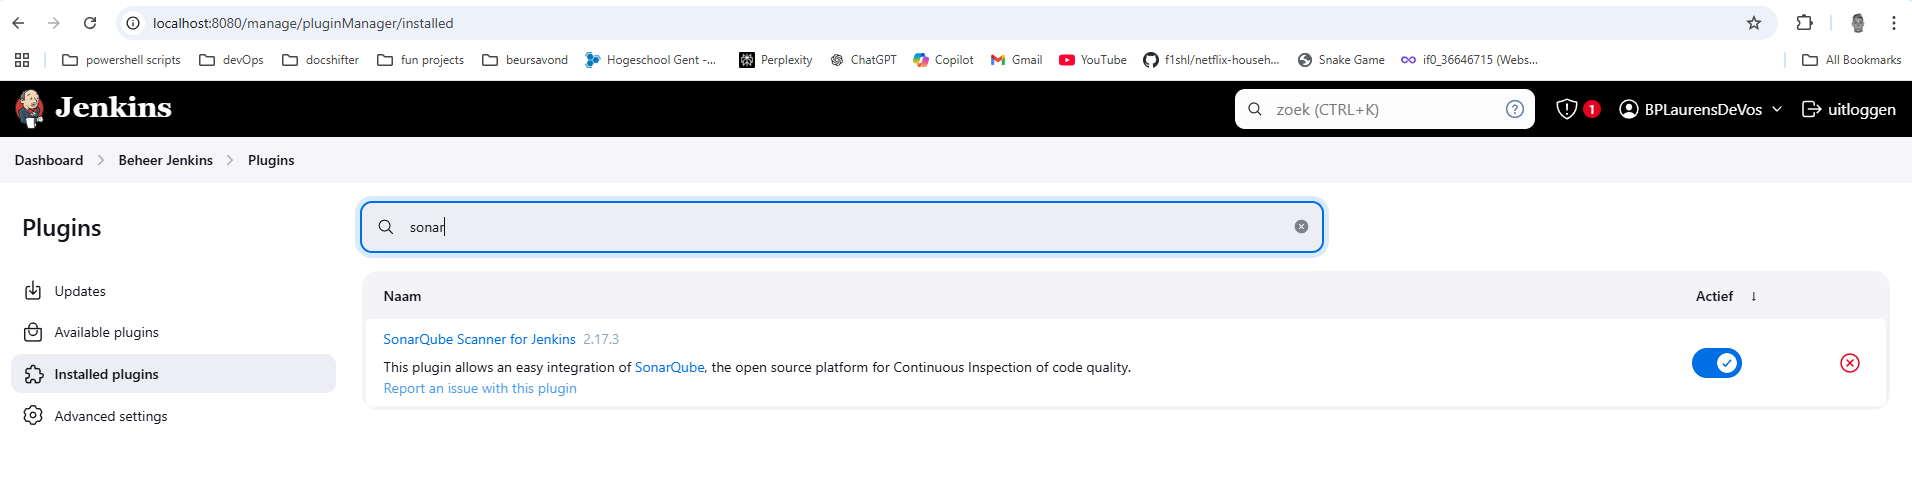
\includegraphics[width=\linewidth]{"C:/Users/laure/Documents/bachelorproef-2024-2025-laurensDeVos/graphics/SonarPlugin.png"}
    \caption{SonarQube scanner plugin geïnstalleerd op de Jenkins server}
    \label{fig:install_Sonar}
\end{figure}

\subsubsection{Configureren van Credentials}

Om de Jenkins-pipeline te laten werken, zijn credentials toegevoegd om toegang te geven tot GitHub en SonarCloud. Dit proces is vergelijkbaar met het configureren van GitHub Secrets in GitHub Actions. De configuratie werd uitgevoerd als volgt:

\begin{enumerate}
    \item \textbf{Toegang tot Credential Management}:
    Ga naar \texttt{Manage Jenkins > Credentials > System > Global Credentials}.
    \item \textbf{Toevoegen van credentials}:
    Voeg de volgende credentials toe als secret text:
    \begin{itemize}
        \item \textbf{GITHUB\_ACTOR}: GitHub-gebruikersnaam.
        \item \textbf{PAT\_TOKEN}: GitHub Personal Access Token, aangemaakt met de rechten \texttt{repo}, \texttt{read:packages}, en \texttt{write:packages}.
        \item \textbf{SONAR\_TOKEN}: Authenticatietoken voor SonarCloud, gegenereerd via \texttt{My Account > Security} in SonarCloud.
    \end{itemize}
    \item \textbf{Bevestiging van credentials}:
    Controleer of de credentials correct zijn opgeslagen. Het overzicht is beschikbaar in de \texttt{Global Credentials}-lijst.
\end{enumerate}

\begin{figure}[h!]
    \centering
    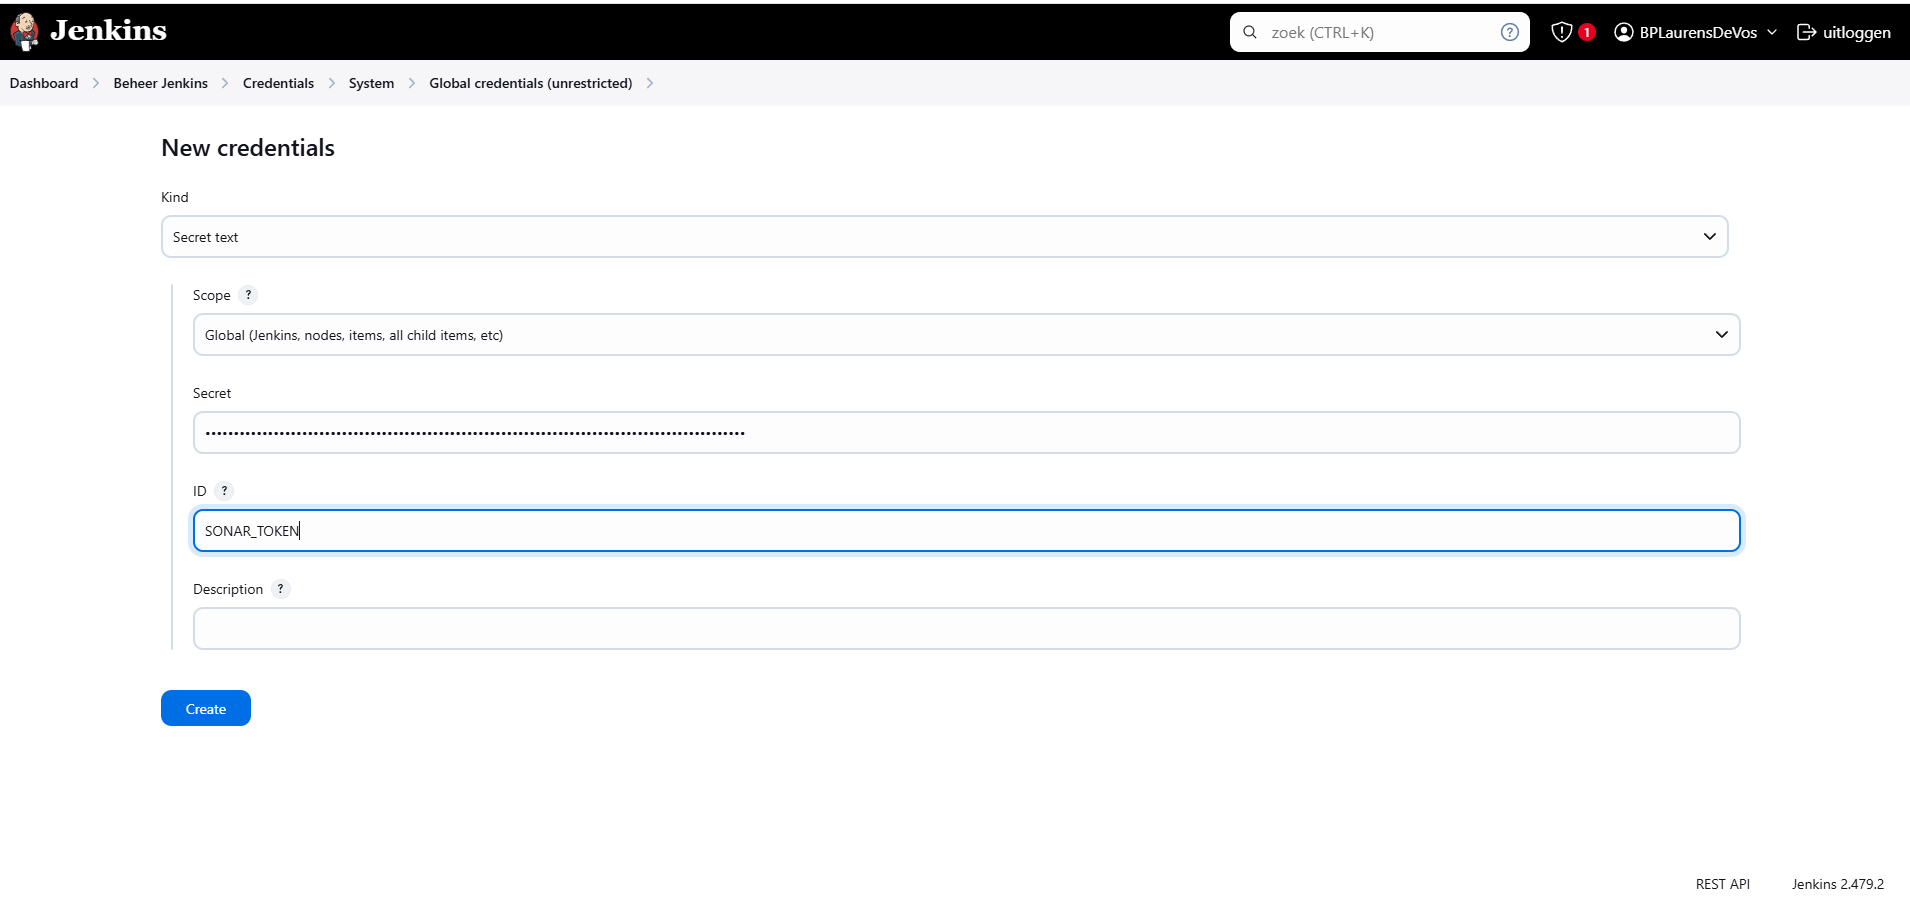
\includegraphics[width=\linewidth]{"C:/Users/laure/Documents/bachelorproef-2024-2025-laurensDeVos/graphics/addCredentials.png"}
    \caption{Toevoegen van credentials in Jenkins.}
    \label{fig:add_credentials}
\end{figure}

\begin{figure}[h!]
    \centering
    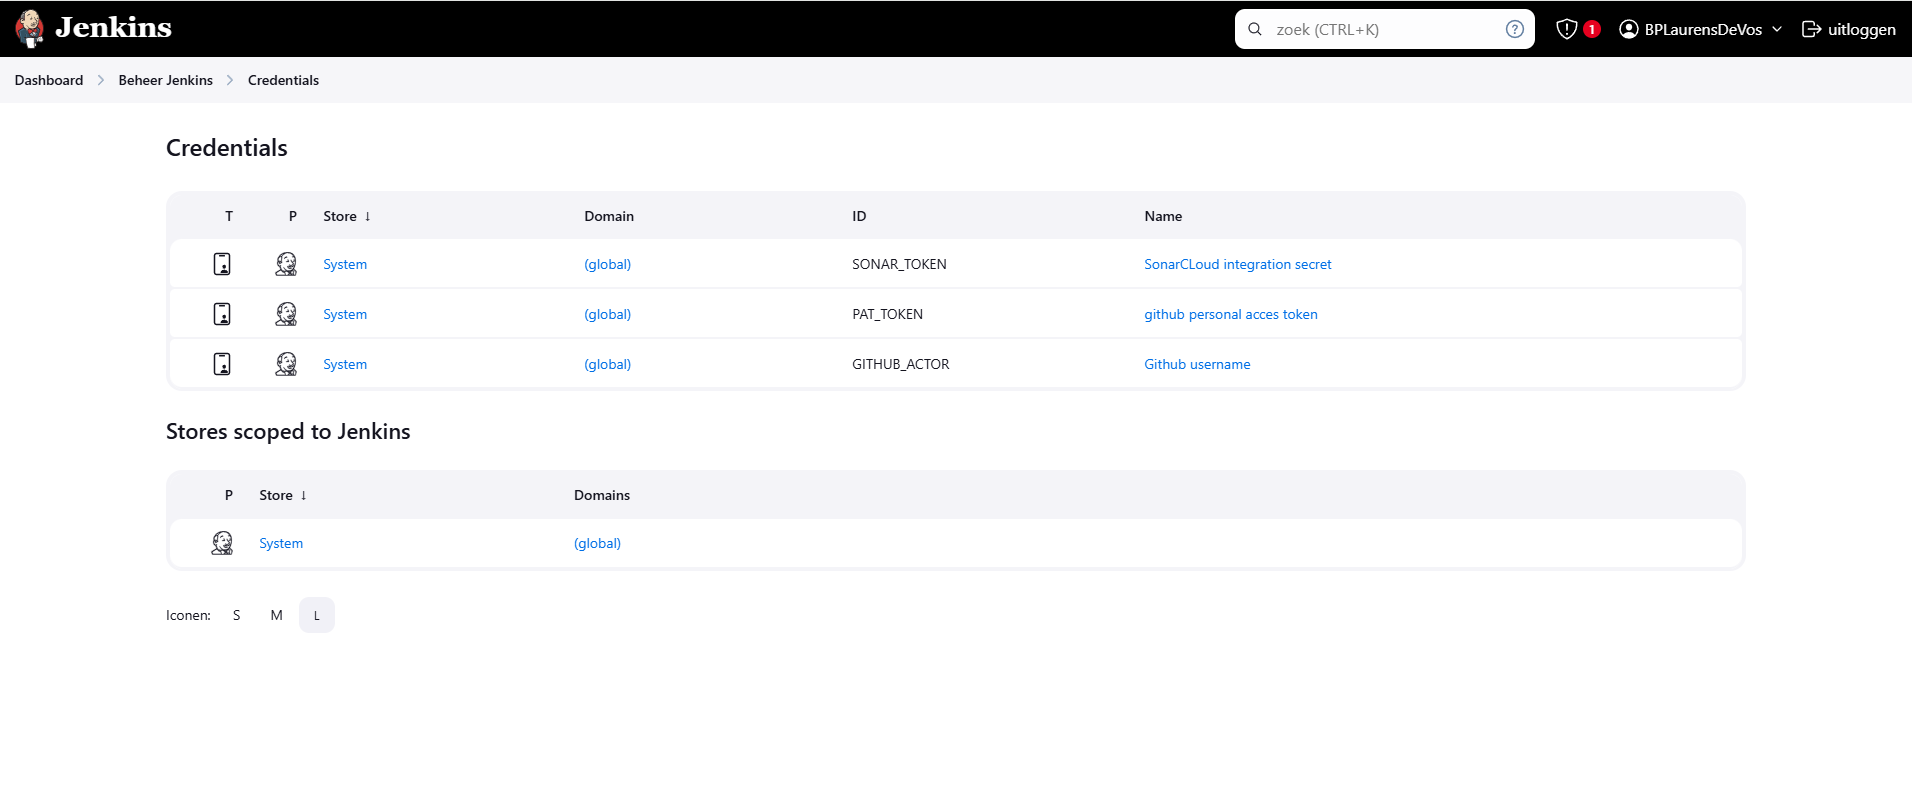
\includegraphics[width=\linewidth]{"C:/Users/laure/Documents/bachelorproef-2024-2025-laurensDeVos/graphics/overzichtCred.png"}
    \caption{Overzicht van geconfigureerde credentials in Jenkins.}
    \label{fig:overview_credentials}
\end{figure}

\subsubsection{Configuratie van de Jenkins Pipeline}

De configuratie van de Jenkins pipeline volgt een vergelijkbare aanpak als de implementatie in GitHub Actions. De Jenkinsfiles voor alle repositories (\texttt{Repo1} tot en met \texttt{Repo5}) zijn gebaseerd op een gestandaardiseerd formaat. Het doel is om een consistent CI/CD-proces te creëren dat kan worden vergeleken met de workflows in Actions.

\paragraph{Aanmaak van de Jenkins Pipeline}

Voor elk van de repositories is een Jenkins pipeline aangemaakt in de Jenkins webinterface. Hier zijn de stappen die zijn gevolgd:

\begin{enumerate} 
    \item Navigeer naar het Jenkins Dashboard:
    Open de Jenkins webinterface en klik op \texttt{New Item} in het dashboard.
    \item Geef een naam aan de pipeline:  
    Voer een unieke naam in voor de pipeline, bijvoorbeeld \texttt{Repo1}, en selecteer het itemtype \texttt{Pipeline}. Klik vervolgens op \texttt{OK}.
    
    \item Configureer de repository in de configuratiepagina:
    \begin{itemize}
        \item Navigeer naar de sectie \texttt{Pipeline}.
        \item Selecteer \texttt{Pipeline script from SCM} als de bron.
        \item Configureer de Git-repository-URL (bijvoorbeeld \texttt{https://github.com/BPLaurensDeVos/repo1}).
        \item Specificeer de branch (\texttt{main}) en het pad naar de Jenkinsfile (\texttt{Jenkinsfile}).
    \end{itemize}
    
    \item Klik op \texttt{Save} om de configuratie van de pipeline op te slaan.
\end{enumerate}   

\paragraph{Algemene structuur van de Jenkinsfile}
De Jenkinsfiles maken gebruik van declarative pipelines, waarin de stappen voor elke repository gedefinieerd zijn in afzonderlijke \texttt{stages}. De Jenkinsfiles worden gedefinieerd in de root map van de repository. De algemene structuur bestaat uit:
\begin{itemize}
    \item Het configureren van tools zoals Maven en JDK.
    \item Het ophalen van de broncode via Git.
    \item Het controleren van afhankelijkheden.
    \item Het bouwen, testen en publiceren van artefacten.
    \item Integratie met SonarCloud voor codekwaliteit.
\end{itemize}

\subparagraph{Tools configuratie}
\begin{verbatim}
        
        tools {
            maven 'Maven3'
            jdk 'jdk17'
        }
        

\end{verbatim}

\begin{itemize}
    \item \textbf{Maven}: Geeft aan dat Maven versie 3 wordt gebruikt als buildtool. Deze is vooraf geconfigureerd in Jenkins onder \texttt{Manage Jenkins > Global Tool Configuration}.
    \item \textbf{JDK}: Specificeert dat JDK versie 17 wordt gebruikt, wat compatibel is met de codebase van het project. Deze versie is nodig voor het compileren van de Java-code.
\end{itemize}

\begin{figure}[h!]
    \centering
    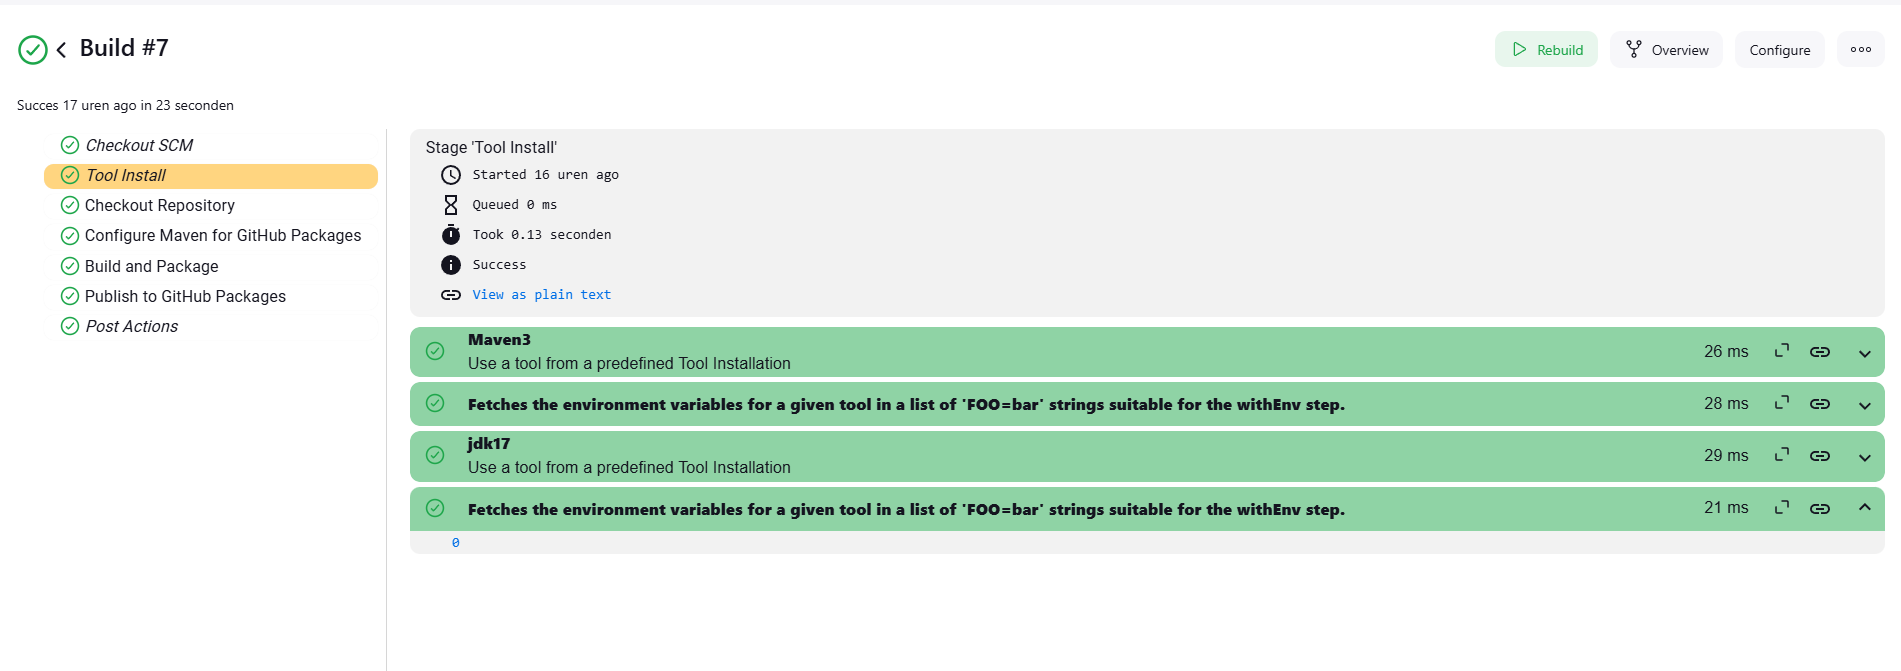
\includegraphics[width=\linewidth]{"C:/Users/laure/Documents/bachelorproef-2024-2025-laurensDeVos/graphics/toolInstall.png"}
    \caption{De uitvoer van de tool installatie in de pipeline.}
\end{figure}

\subparagraph{Environment configuratie}
\begin{verbatim}
    
        environment {
            GITHUB_ACTOR = credentials('GITHUB_ACTOR')
            GITHUB_TOKEN = credentials('PAT_TOKEN')
        }
  
\end{verbatim}

\begin{itemize}
    \item \textbf{GITHUB\_ACTOR}: Verwijst naar de GitHub-gebruikersnaam. Deze wordt opgeslagen als een credential in Jenkins onder \texttt{Manage Jenkins > Credentials}.
    \item \textbf{PAT\_TOKEN}: Dit is een Personal Access Token (PAT) dat wordt gebruikt voor authenticatie bij GitHub. Het token biedt toegang tot de repository en stelt Maven in staat om artefacten naar GitHub Packages te publiceren.
\end{itemize}

\subparagraph{Stages uitleg}
\textbf{Stage 1: Checkout Repository}
Deze stap zorgt voor het ophalen van de meest recente broncode van de repository door gebruik te maken van \textbf{checkout scm}.

\begin{verbatim}
    
    stage('Checkout Repository') {
        steps {
            echo "Checking out repository..."
            checkout scm
        }
    }

\end{verbatim}

\begin{figure}[h!]
    \centering
    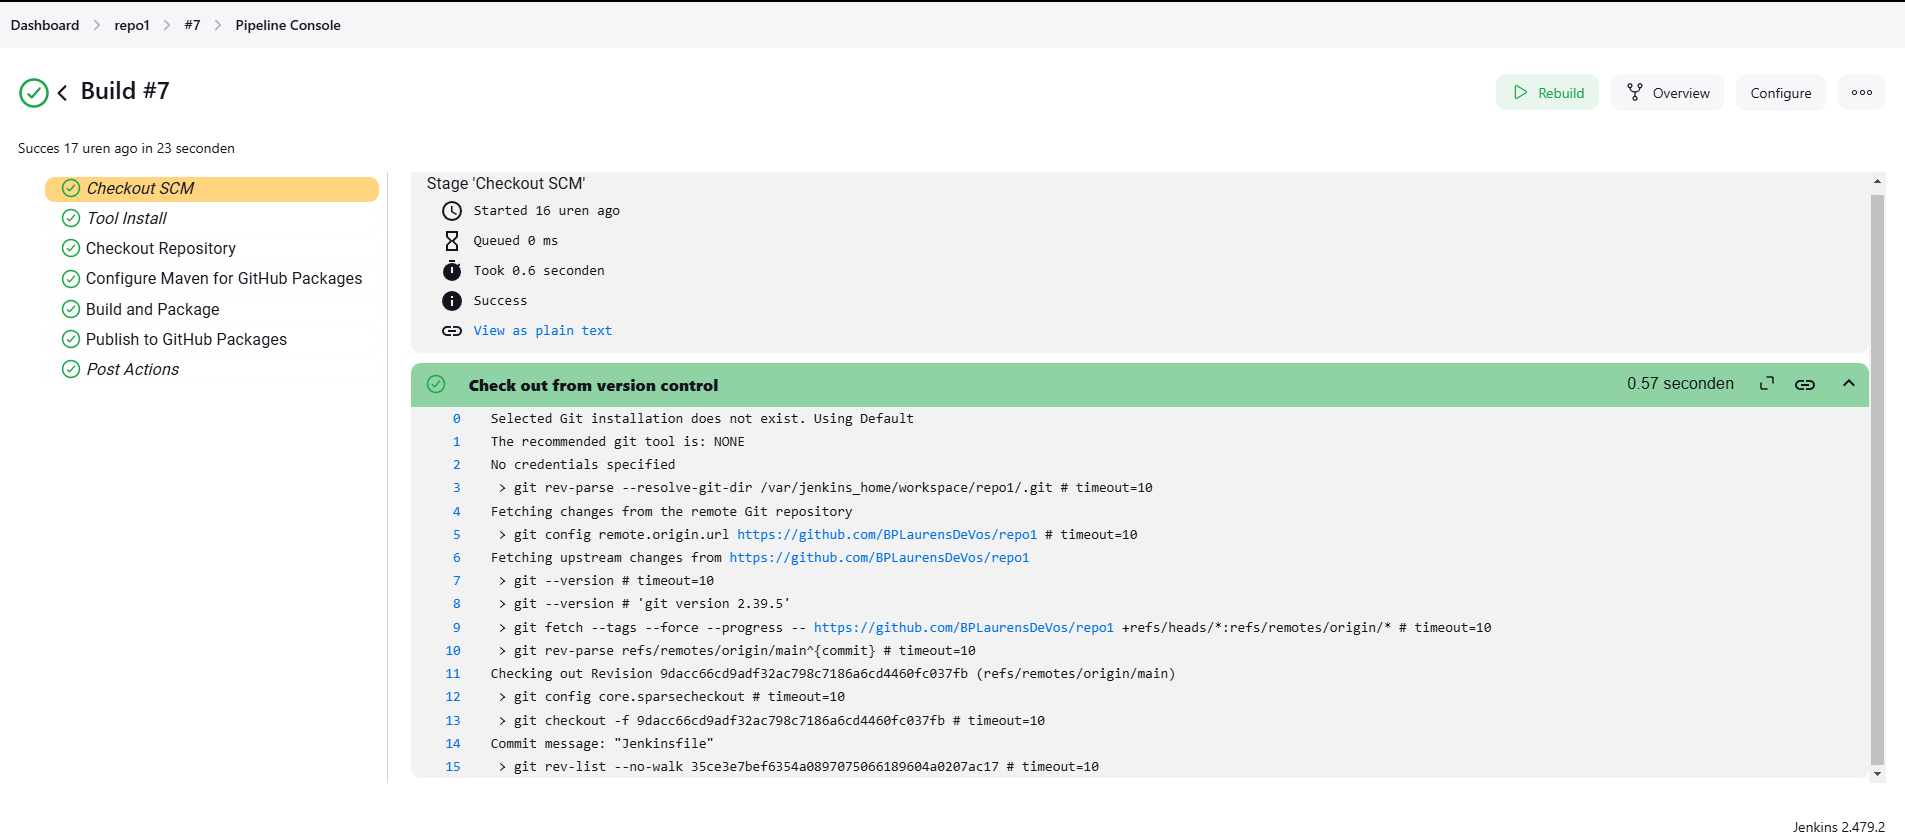
\includegraphics[width=\linewidth]{"C:/Users/laure/Documents/bachelorproef-2024-2025-laurensDeVos/graphics/checkoutscm.png"}
    \caption{De uitvoer tijdens het ophalen van de meest recente broncode van GitHub}
\end{figure}


\textbf{Stage 2: Configure Maven for GitHub Packages}
Deze stap zorgt voor het aanmaken van settings.xml die authenticatiegegevens bevat om toegang te krijgen tot Github Packages.

\begin{verbatim}
    
stage('Configure Maven for GitHub Packages') {
    steps {
        echo "Configuring Maven for GitHub Packages..."
        sh """
        mkdir -p ~/.m2
        echo "<settings xmlns='http://maven.apache.org/SETTINGS/1.0.0'>
            <servers>
              <server>
                <id>github</id>
                <username>${env.GITHUB_ACTOR}</username>
                <password>${env.GITHUB_TOKEN}</password>
              </server>
            </servers>
        </settings>" > ~/.m2/settings.xml
        """
    }
}
    
\end{verbatim}

\begin{figure}[h!]
    \centering
    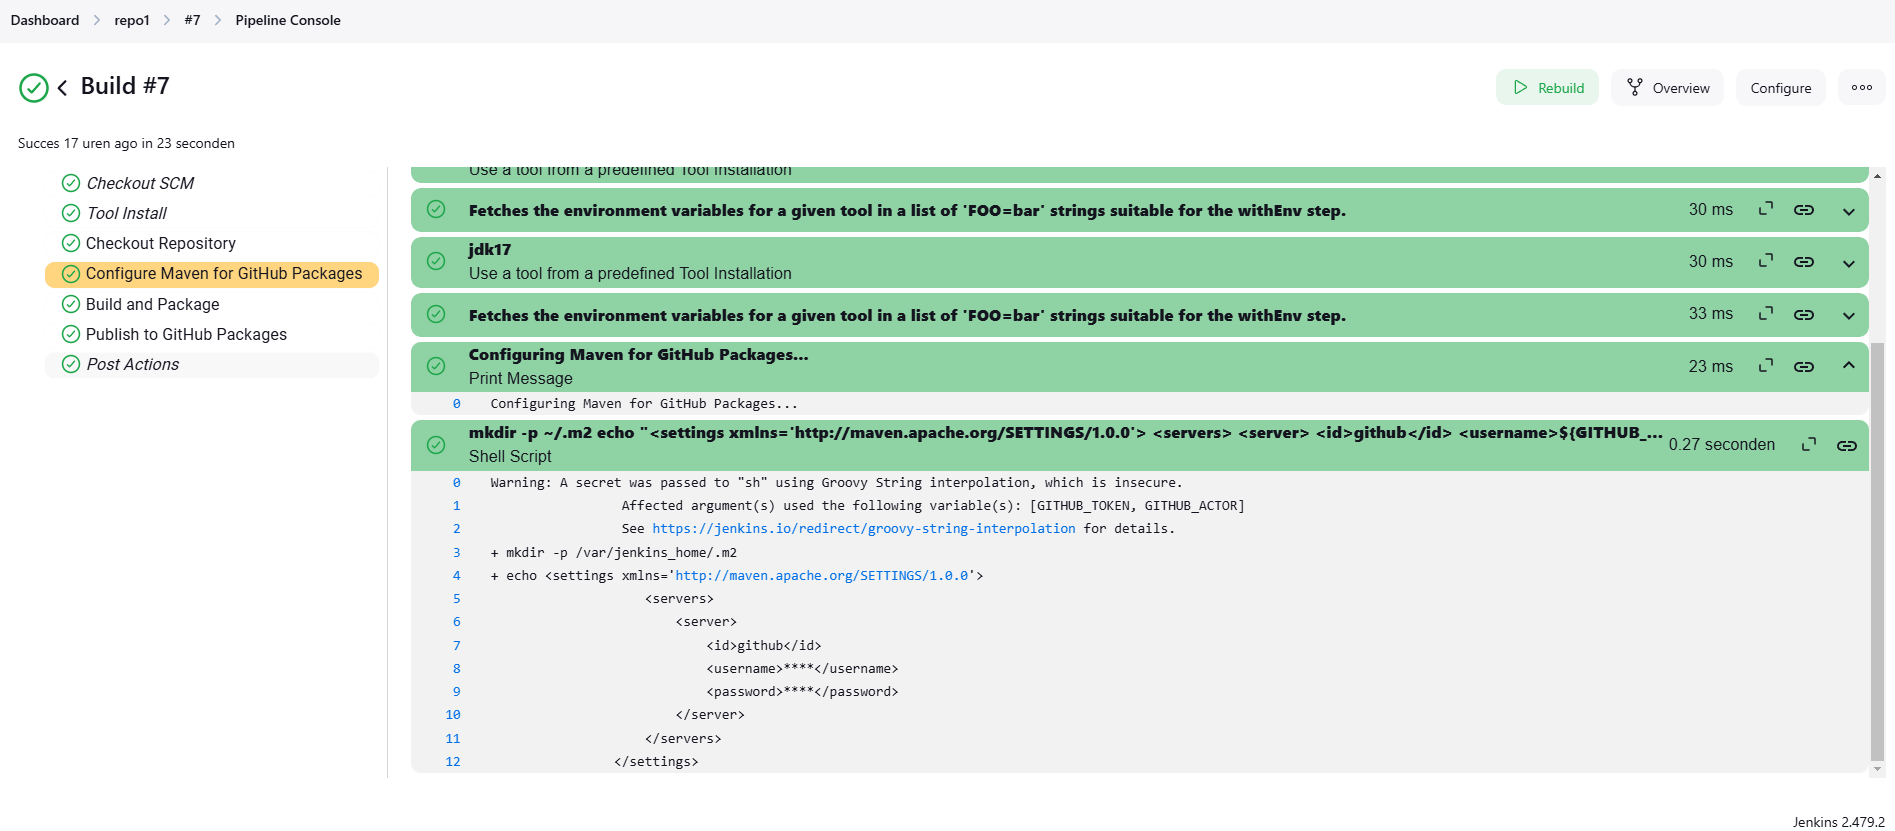
\includegraphics[width=\linewidth]{"C:/Users/laure/Documents/bachelorproef-2024-2025-laurensDeVos/graphics/confmvn.png"}
    \caption{De uitvoer van stage2.}
\end{figure}


\textbf{Stage 3: Build and Package}
Net zoals bij github actions wordt hetzelfde commando gebruikt om de java-code te compileren en testen.

\begin{verbatim}
    
    stage('Build and Package') {
        steps {
            echo "Building and packaging the project..."
            sh "mvn clean package"
        }
    }

    
\end{verbatim}

\begin{figure}[h!]
    \centering
    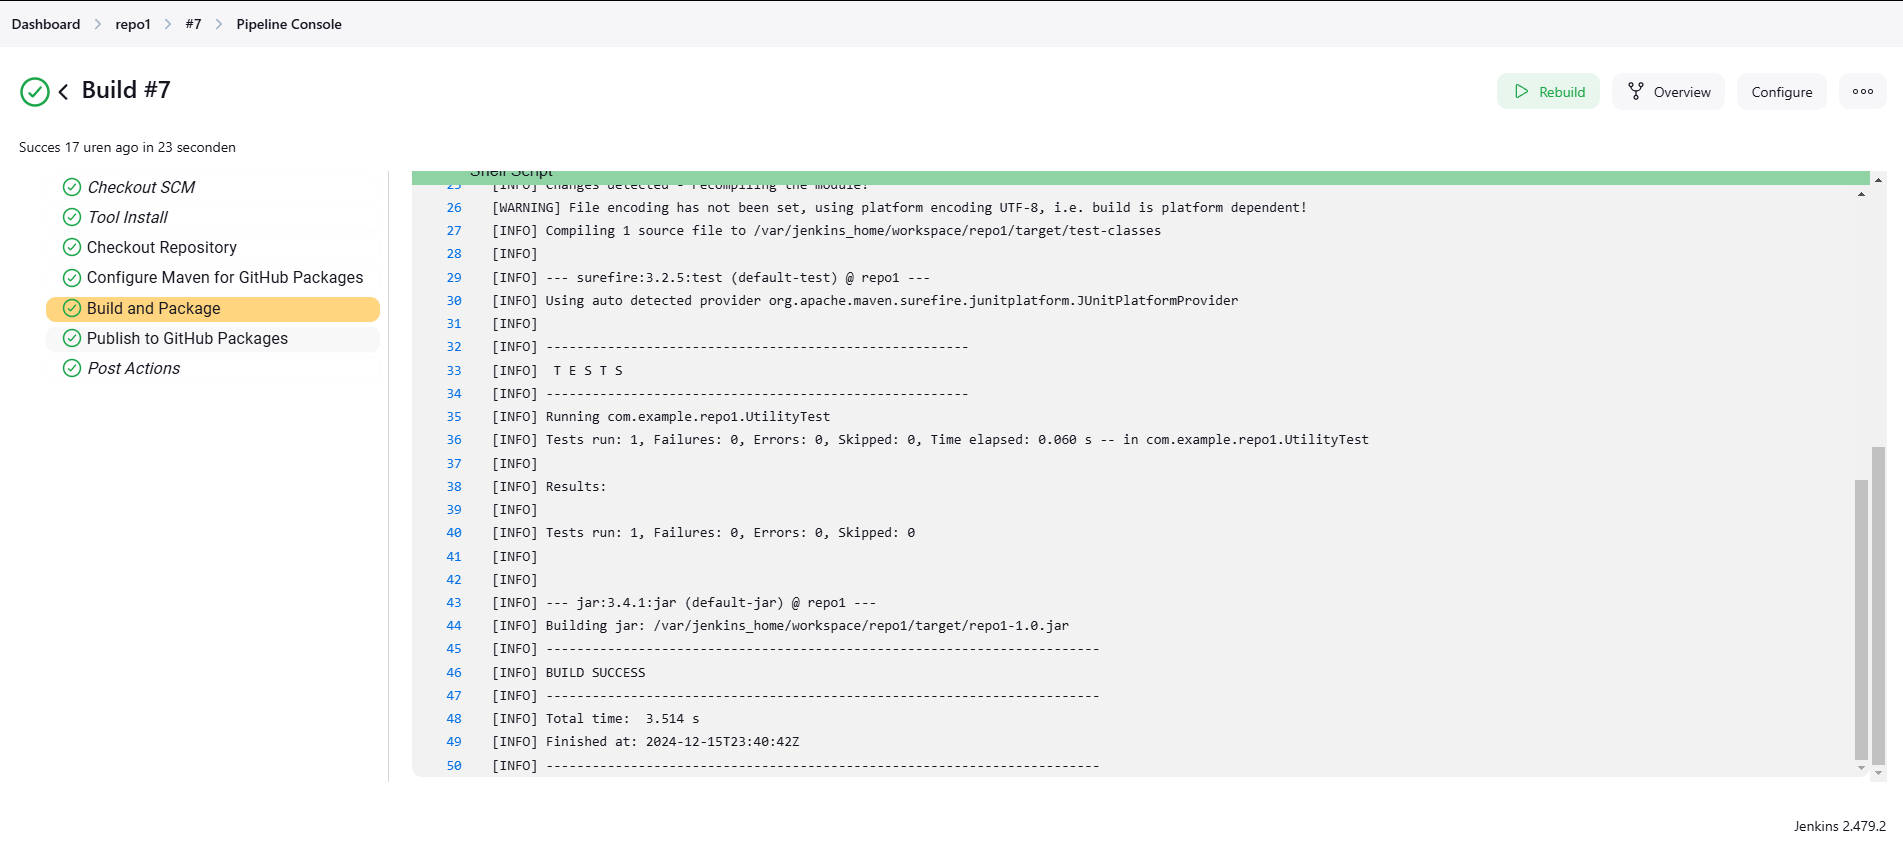
\includegraphics[width=\linewidth]{"C:/Users/laure/Documents/bachelorproef-2024-2025-laurensDeVos/graphics/buildpackagejenkins.png"}
    \caption{build succes toont aan dat de code is opgebouwd en getest.}
\end{figure}

\textbf{Stage 4: Publish to GitHub Packages}
Publiceert het gebouwde JAR-bestand van de vorige stage naar de GitHub Package Registry. 

\begin{verbatim}
    
    stage('Publish to GitHub Packages') {
        steps {
            echo "Publishing to GitHub Packages..."
            sh "mvn deploy"
        }
    }
    
\end{verbatim}

\begin{figure}[h!]
    \centering
    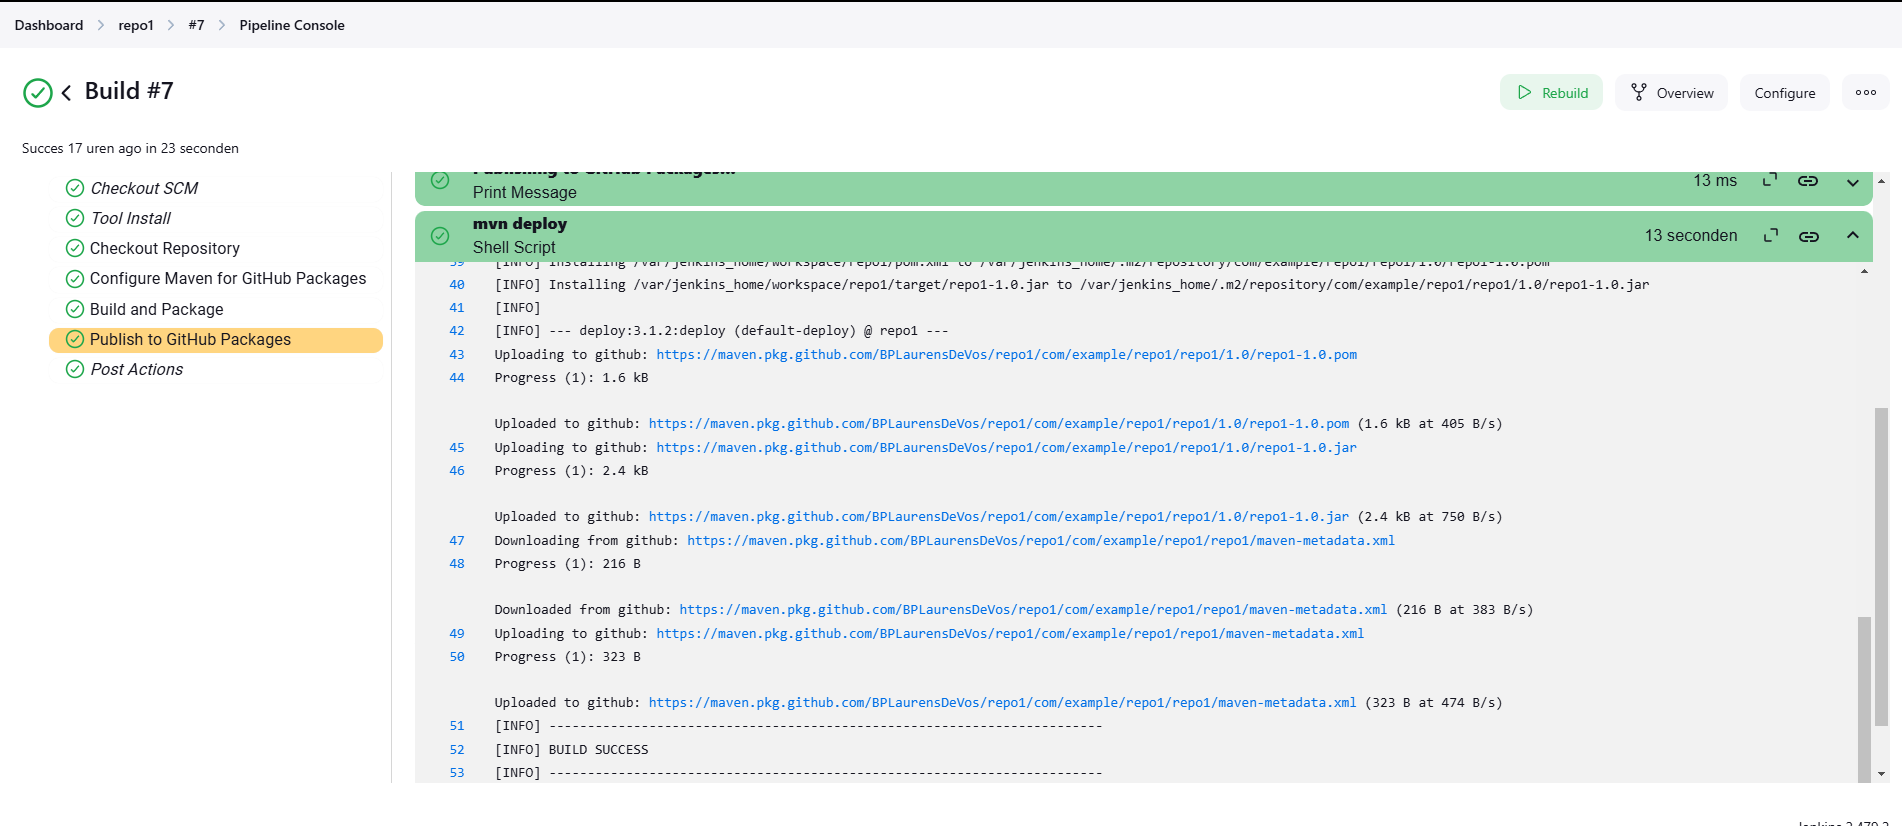
\includegraphics[width=\linewidth]{"C:/Users/laure/Documents/bachelorproef-2024-2025-laurensDeVos/graphics/publiceerjenkins.png"}
    \caption{Het artefact bestand wordt opgeladen in de GitHub Package Registry.}
\end{figure}

\subparagraph{Post-sectie uitleg}
Door deze code toe te voegen aan het bestand krijgen we feedback bij de uitvoering van de pipeline. 

\begin{verbatim}
    
    post {
        success {
            echo "Pipeline executed successfully for Repo1!"
        }
        failure {
            echo "Pipeline failed. Please check the logs for errors."
        }
    }

\end{verbatim}

\begin{figure}[h!]
    \centering
    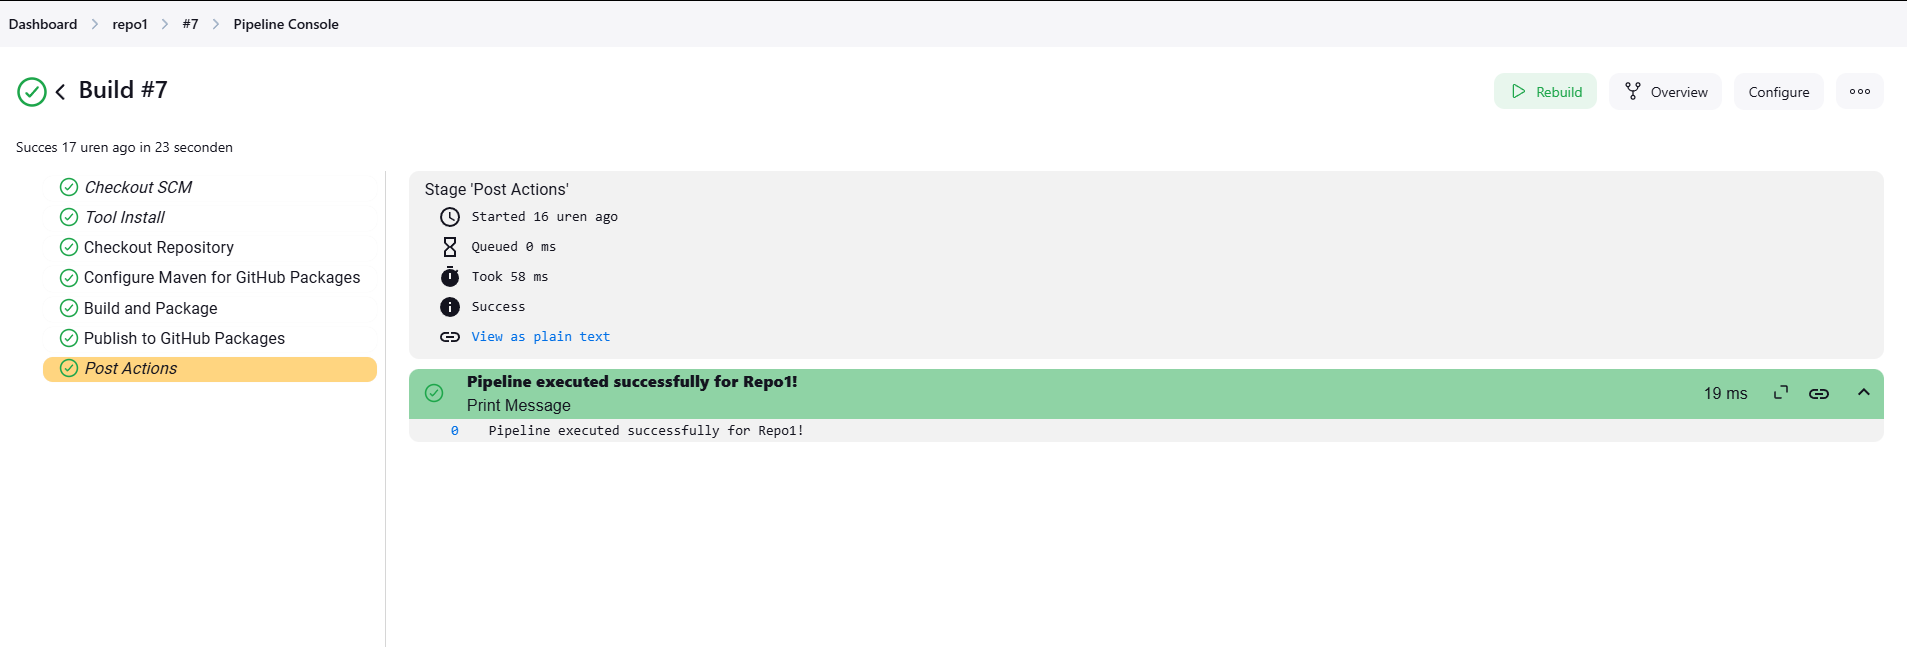
\includegraphics[width=\linewidth]{"C:/Users/laure/Documents/bachelorproef-2024-2025-laurensDeVos/graphics/post.png"}
    \caption{Een succesmelding wordt gegeven wanneer alle stages zonder fouten worden uitgevoerd.}
\end{figure}

\begin{figure}[h!]
    \centering
    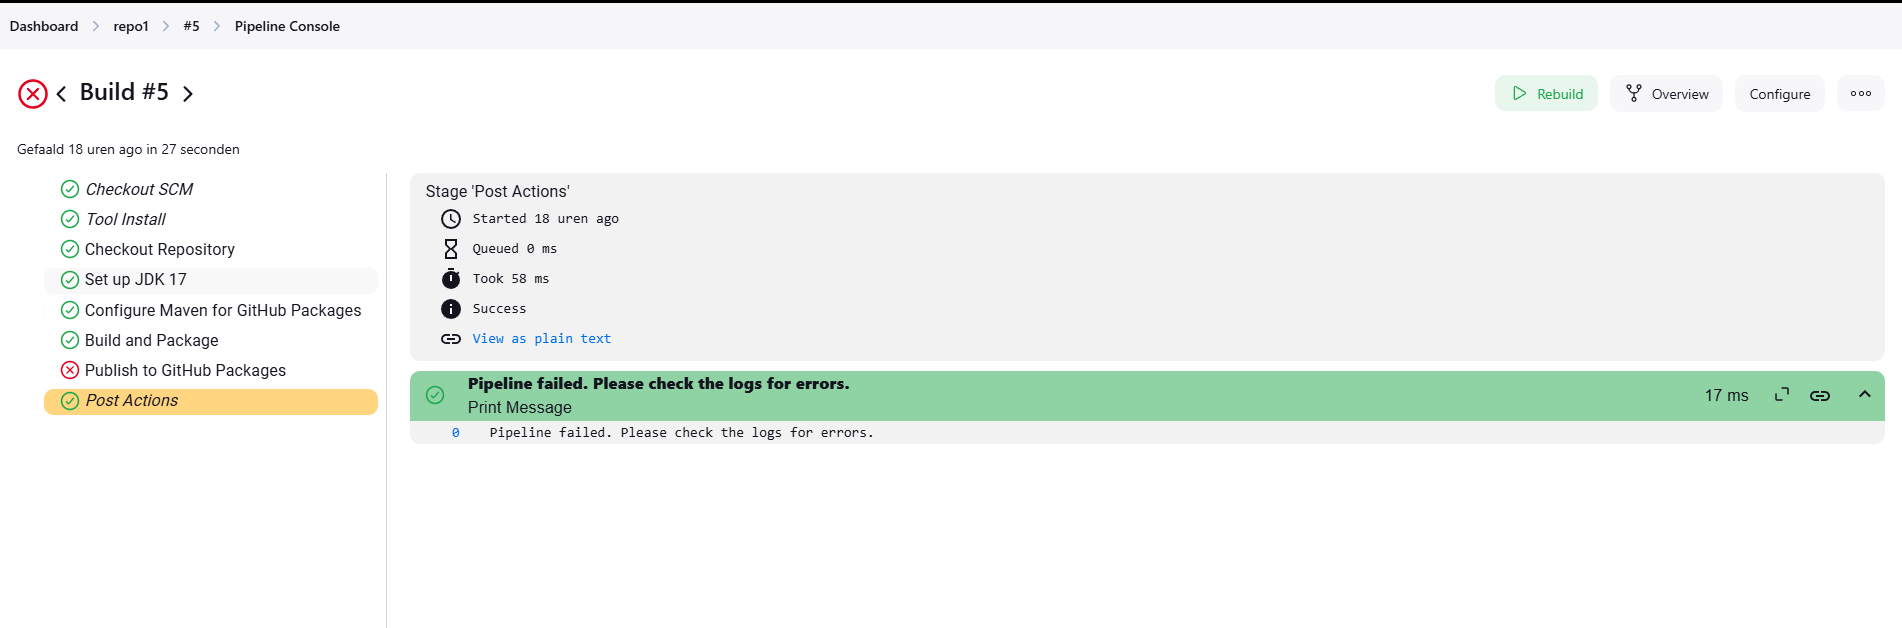
\includegraphics[width=\linewidth]{"C:/Users/laure/Documents/bachelorproef-2024-2025-laurensDeVos/graphics/postfout.png"}
    \caption{Een foutmelding wordt gegeven wanneer de pipeline een fout tegenkomt.}
\end{figure}

\subparagraph{Jenkinsfile voor repo1} 

\begin{verbatim}
    
    pipeline {
        agent any
        
        tools {
            maven 'Maven3'
            jdk 'jdk17'
        }
        
        environment {
            GITHUB_ACTOR = credentials('GITHUB_ACTOR')
            GITHUB_TOKEN = credentials('PAT_TOKEN')
        }
        
        stages {
            stage('Checkout Repository') {
                steps {
                    echo "Checking out repository..."
                    checkout scm
                }
            }
            
            stage('Configure Maven for GitHub Packages') {
                steps {
                    echo "Configuring Maven for GitHub Packages..."
                    sh """
                    mkdir -p ~/.m2
                    echo "<settings xmlns='http://maven.apache.org/SETTINGS/1.0.0'>
                        <servers>
                          <server>
                            <id>github</id>
                            <username>${env.GITHUB_ACTOR}</username>
                            <password>${env.GITHUB_TOKEN}</password>
                          </server>
                        </servers>
                    </settings>" > ~/.m2/settings.xml
                    """
                }
            }
            
            stage('Build and Package') {
                steps {
                    echo "Building and packaging the project..."
                    sh "mvn clean package"
                }
            }
            
            stage('Publish to GitHub Packages') {
                steps {
                    echo "Publishing to GitHub Packages..."
                    sh "mvn deploy"
                }
            }
        }
        
        post {
            success {
                echo "Pipeline executed successfully for Repo1!"
            }
            failure {
                echo "Pipeline failed. Please check the logs for errors."
            }
        }
    }

    
\end{verbatim}

\paragraph{Specifieke Configuraties voor downstream repositories}

\subparagraph{Configuratie voor \texttt{Repo2}}
Net zoals in GitHub Actions heeft \texttt{Repo2} een afhankelijkheid van \texttt{Repo1}. De pipeline voor \texttt{Repo2} controleert eerst of het artefact van \texttt{Repo1} beschikbaar is in GitHub Packages. Indien het artefact ontbreekt, wordt de Jenkins pipeline van \texttt{Repo1} getriggerd om het artefact te genereren. Vervolgens bouwt, test, en publiceert de pipeline het artefact van \texttt{Repo2}. 

Hieronder volgt een overzicht van de extra stappen in de Jenkinsfile voor repo2 tot en met repo5:

\begin{verbatim}
    stage('Artifact Check & Trigger') {
        steps {
            script {
                def statusCode = sh(
                script: "curl -L -u ${GITHUB_ACTOR}:${GITHUB_TOKEN} -s -o /dev/null -w '%{http_code}' ${REPO1_URL}",
                returnStdout: true
                ).trim()
                
                if (statusCode != '200') {
                    echo "Artifact missing. Triggering Repo1 Jenkins pipeline..."
                    build job: 'repo1', wait: true, propagate: true
                } else {
                    echo "Artifact is available. Proceeding with build."
                }
            }
        }
    }
\end{verbatim}

\textbf{Wat doet deze stap?}
\begin{itemize}
    \item Controleert de beschikbaarheid van het artefact van \texttt{repo1} met behulp van een HTTP-verzoek naar GitHub Packages.
    \item Start de Jenkins pipeline van \texttt{repo1} indien het artefact niet beschikbaar is met behulp van het \textbf{build job} commando.
\end{itemize}

\textbf{Waarom is deze stap belangrijk?}
\begin{itemize}
    \item Zorgt ervoor dat de afhankelijkheden correct worden beheerd en downstream builds niet falen vanwege ontbrekende artefacten.
    \item Dit mechanisme is essentieel voor het beheren van complexe afhankelijkheden tussen meerdere repositories.
\end{itemize}

Afbeelding \ref{fig:artifact_check_trigger} toont dat de pipeline in \texttt{Repo1} werd gestart door \texttt{Repo2}. Vervolgens werd \texttt{Repo2} getriggerd door \texttt{Repo3}, die op zijn beurt werd geactiveerd door \texttt{Repo4}, waarna het proces uiteindelijk begon bij \texttt{Repo5}.

\begin{figure}[h!]
    \centering
    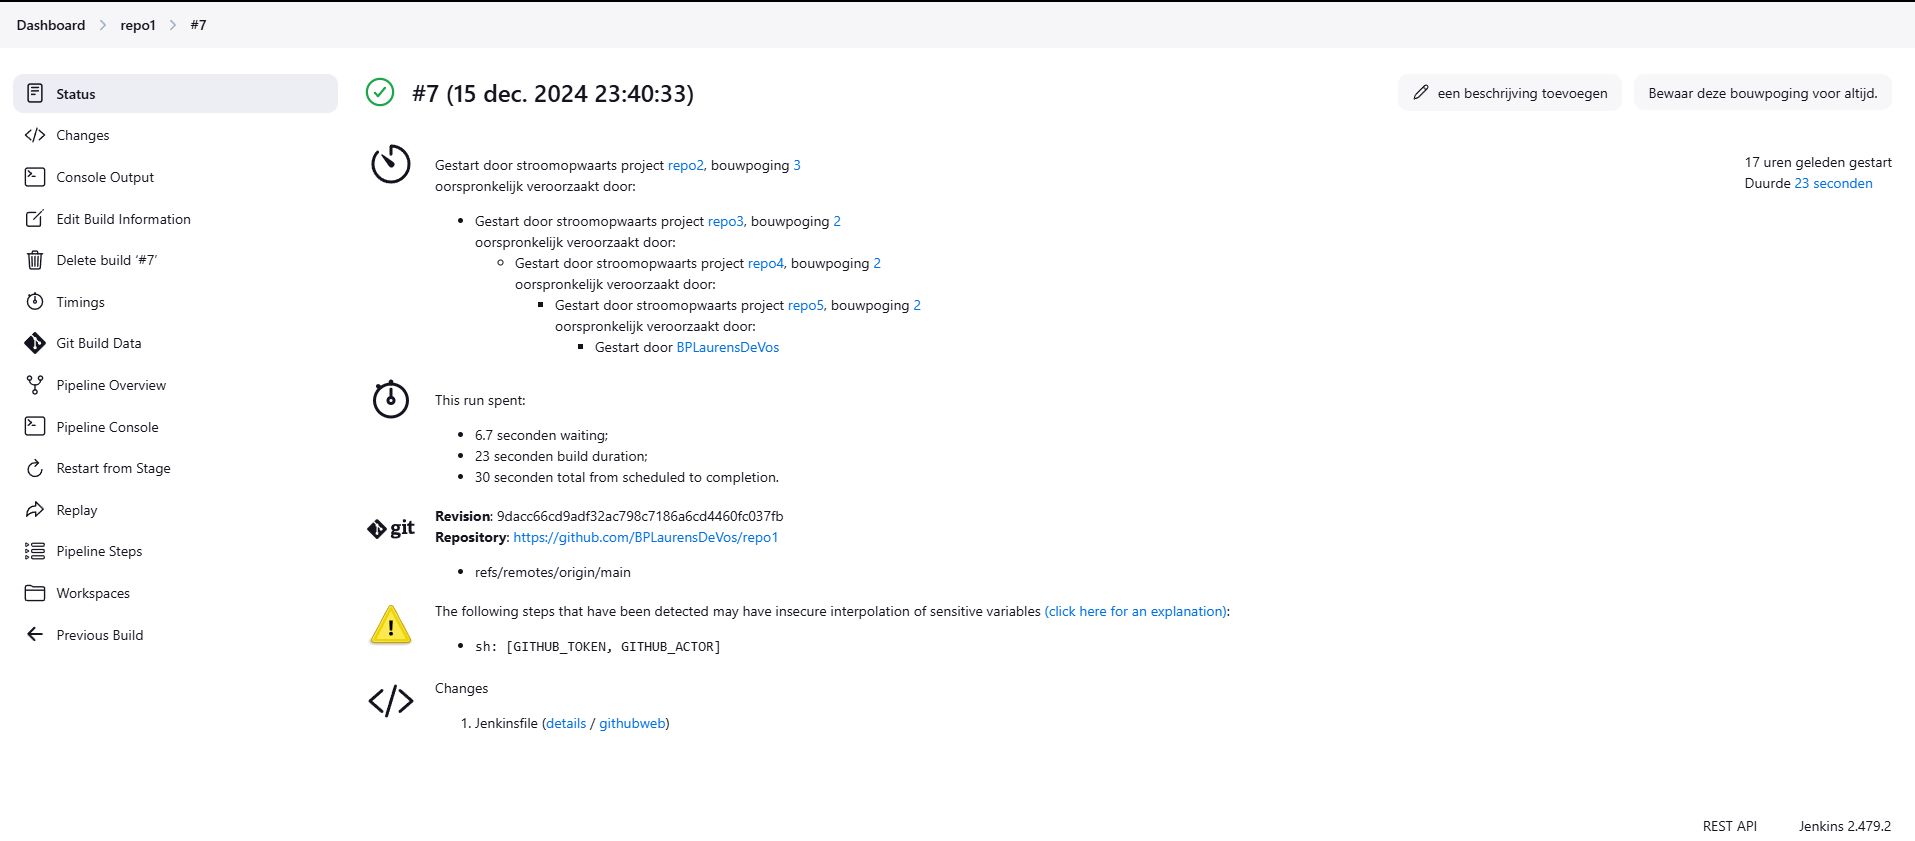
\includegraphics[width=\linewidth]{"C:/Users/laure/Documents/bachelorproef-2024-2025-laurensDeVos/graphics/triggerjenkins.png"}
    \label{fig:artifact_check_trigger}
\end{figure}

\subparagraph{Configuratie voor \texttt{Repo3}, \texttt{Repo4}, en \texttt{Repo5}}
De Jenkinsfiles voor \texttt{Repo3}, \texttt{Repo4}, en \texttt{Repo5} volgen dezelfde logica als \texttt{Repo2}, maar met aangepaste code voor afhankelijkheden. Zo controleert \texttt{Repo3} de beschikbaarheid van het artefact van \texttt{Repo2}.

Voorbeeld van de \texttt{Artifact Check} voor \texttt{Repo3}:

\begin{verbatim}
    stage('Artifact Check & Trigger') {
        steps {
            script {
                def statusCode = sh(
                script: "curl -L -u ${GITHUB_ACTOR}:${GITHUB_TOKEN} -s -o /dev/null -w '%{http_code}' ${REPO2_URL}",
                returnStdout: true
                ).trim()
                
                if (statusCode != '200') {
                    echo "Artifact missing. Triggering Repo2 Jenkins pipeline..."
                    build job: 'repo2', wait: true, propagate: true
                } else {
                    echo "Artifact is available. Proceeding with build."
                }
            }
        }
    }
\end{verbatim}

\paragraph{SonarCloud Integratie}
Net zoals in GitHub Actions wordt SonarCloud gebruikt om de codekwaliteit te bewaken. Dit gebeurt met de \texttt{SonarQube Scanner for Jenkins}-plugin. De configuratie is gedetailleerd beschreven in sectie \ref{subsec:voorbereidingvanhetproject} en wordt herhaald in de Jenkins pipeline met de volgende stap:

\begin{verbatim}
    stage('SonarCloud Scan') {
        steps {
            withSonarQubeEnv('SonarQube') {
                sh 'mvn sonar:sonar'
            }
        }
    }
\end{verbatim}

\textbf{Waarom belangrijk?}
\begin{itemize}
    \item Detecteert potentiële kwetsbaarheden in de code.
    \item Zorgt voor naleving van kwaliteitsstandaarden.
\end{itemize}

Afbeelding \ref{fig:sonarcloud_scan} toont de succesvolle uitvoering van een SonarCloud-scan in de omgeving op sonarcloud.

\begin{figure}[h!]
    \centering
    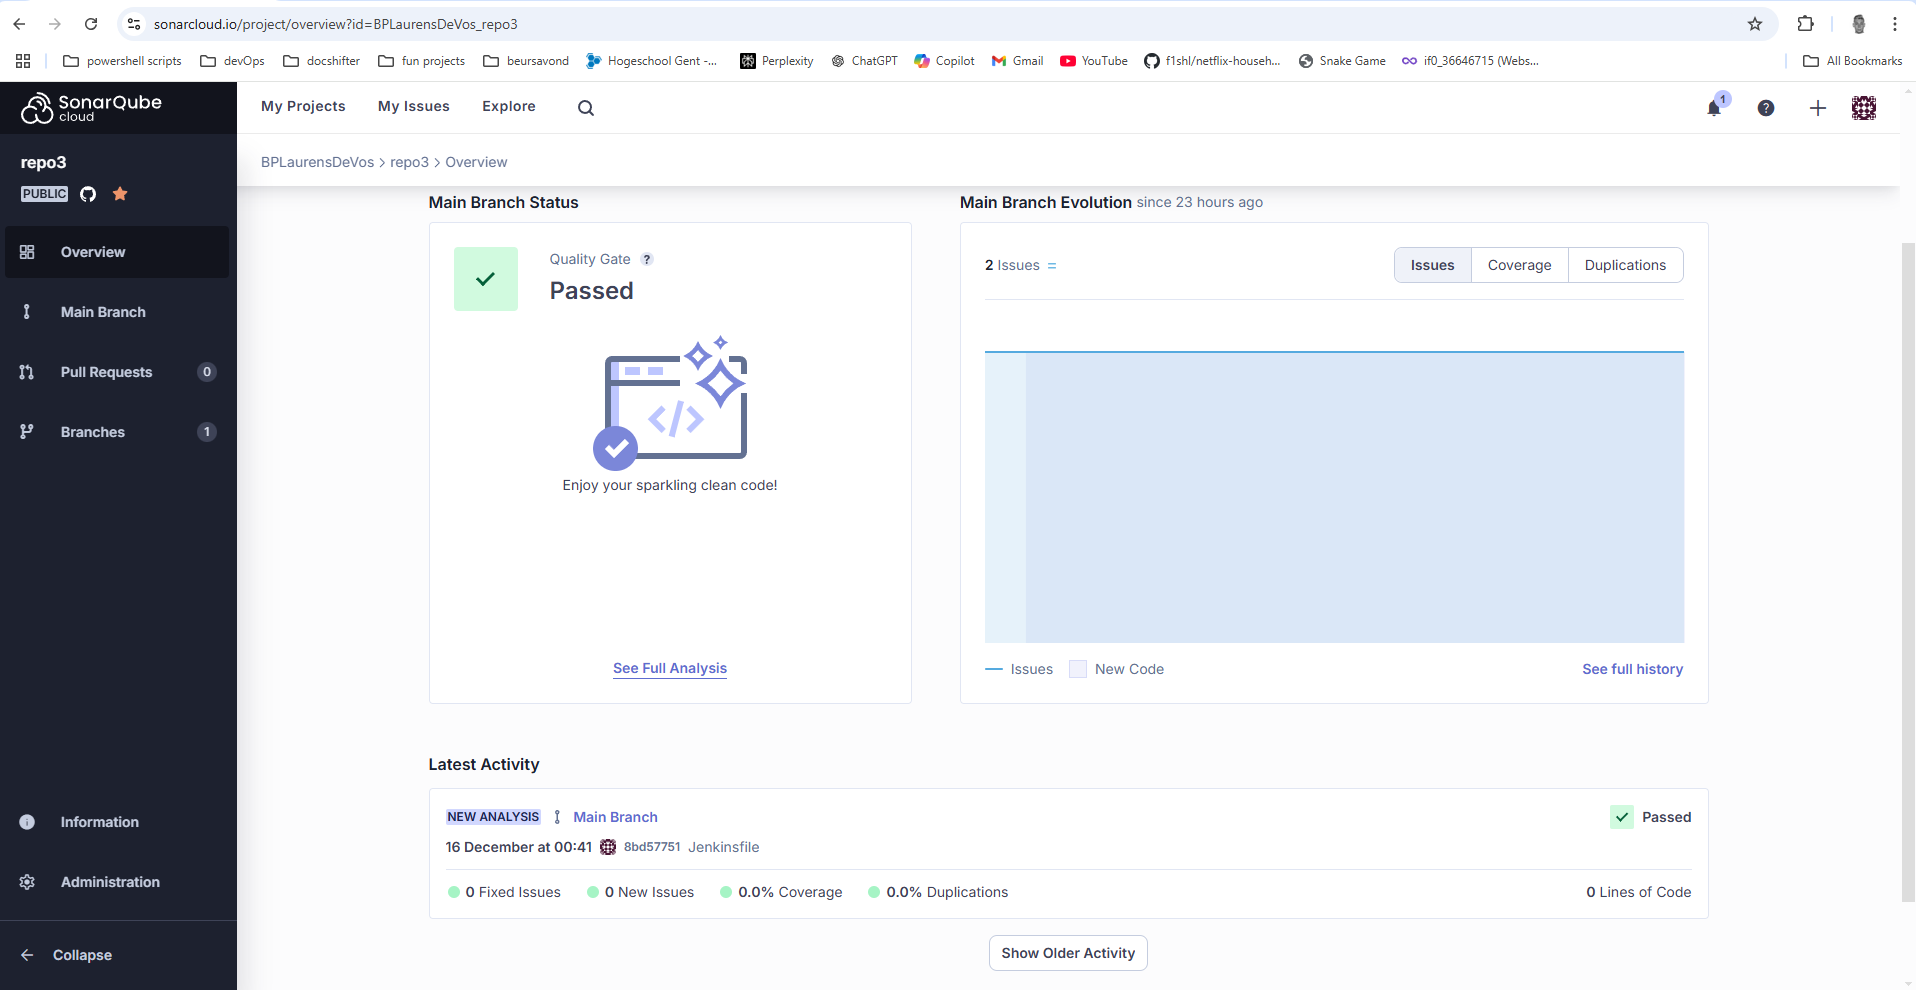
\includegraphics[width=\linewidth]{"C:/Users/laure/Documents/bachelorproef-2024-2025-laurensDeVos/graphics/sonarcloudjenkins.png"}
    \caption{Succesvolle SonarCloud scan opgestart door het Jenkinsfile.}
    \label{fig:sonarcloud_scan}
\end{figure}

\subparagraph{Jenkinsfile voor repo3} 

\begin{verbatim}
    
    pipeline {
        agent any
        
        tools {
            maven 'Maven3'
            jdk 'jdk17'
        }
        
        environment {
            GITHUB_ACTOR = credentials('GITHUB_ACTOR')
            GITHUB_TOKEN = credentials('PAT_TOKEN')
            SONAR_TOKEN = credentials('SONAR_TOKEN')
            REPO2_URL = "https://maven.pkg.github.com/BPLaurensDeVos/repo2/com/example/repo2/repo2/1.0/repo2-1.0.jar"
        }
        
        stages {
            stage('Checkout') {
                steps {
                    checkout scm
                }
            }
            
            stage('Artifact Check & Trigger') {
                steps {
                    script {
                        def statusCode = sh(
                        script: "curl -L -u ${GITHUB_ACTOR}:${GITHUB_TOKEN} -s -o /dev/null -w '%{http_code}' ${REPO2_URL}",
                        returnStdout: true
                        ).trim()
                        
                        if (statusCode != '200') {
                            echo "Artifact missing. Triggering Repo2 Jenkins pipeline..."
                            build job: 'repo2', wait: true, propagate: true
                        } else {
                            echo "Artifact is available. Proceeding with build."
                        }
                    }
                }
            }
            
            stage('Configure Maven') {
                steps {
                    sh """
                    mkdir -p ~/.m2
                    echo "<settings xmlns='http://maven.apache.org/SETTINGS/1.0.0'
                    xmlns:xsi='http://www.w3.org/2001/XMLSchema-instance'
                    xsi:schemaLocation='http://maven.apache.org/SETTINGS/1.0.0 https://maven.apache.org/xsd/settings-1.0.0.xsd'>
                    <servers>
                      <server>
                        <id>github-repo1</id>
                        <username>${GITHUB_ACTOR}</username>
                        <password>${GITHUB_TOKEN}</password>
                      </server>
                      <server>
                        <id>github-repo2</id>
                        <username>${GITHUB_ACTOR}</username>
                        <password>${GITHUB_TOKEN}</password>
                      </server>
                      <server>
                        <id>github-repo3</id>
                        <username>${GITHUB_ACTOR}</username>
                        <password>${GITHUB_TOKEN}</password>
                      </server>
                    </servers>
                    </settings>" > ~/.m2/settings.xml
                    """
                }
            }
            
            stage('Build and Test') {
                steps {
                    sh 'mvn clean package'
                }
            }
            
            stage('SonarCloud Scan') {
                steps {
                    withSonarQubeEnv('SonarCloud') {
                        sh 'mvn sonar:sonar'
                    }
                }
            }
            
            stage('Deploy to GitHub Packages') {
                steps {
                    sh 'mvn deploy'
                }
            }
        }
        
        post {
            success {
                echo 'Pipeline completed successfully.'
            }
            failure {
                echo 'Pipeline failed.'
            }
        }
    }

   
\end{verbatim}

\subparagraph{Conclusie}
De implementatie van CI/CD-pipelines met Jenkins biedt een flexibel en schaalbaar alternatief voor GitHub Actions. Dankzij het gebruik van Jenkinsfiles en het beheren van afhankelijkheden tussen repositories is een vergelijkbare workflow gecreëerd.


\section{Vergelijkende analyse van Jenkins en Github Actions}

\subsection{Inleiding}
In dit hoofdstuk worden Jenkins en GitHub Actions rechtstreeks met elkaar vergeleken op basis van de resultaten van de Proof-of-Concept (PoC). Door middel van deze analyse wordt beantwoord welke tool het meest geschikt is voor de specifieke behoeften van DocShifter, zoals aangegeven in de centrale onderzoeksvraag.

De vergelijking richt zich op vier kerncriteria:
\begin{itemize}
    \item \textbf{Prestaties}: Evaluatie van de snelheid en efficiëntie van builds in beide tools, met bijzondere aandacht voor eventuele bottlenecks.
    \item \textbf{Beveiliging}: Analyse van hoe beide tools omgaan met het beheer van credentials en toegangsrechten.
    \item \textbf{Automatiseringsefficiëntie}: Vergelijking van de eenvoud en flexibiliteit bij het configureren en beheren van workflows en pipelines.
    \item \textbf{Integratie met bestaande systemen}: Beoordeling van hoe gemakkelijk beide tools kunnen worden geïntegreerd met externe systemen en technologieën, zoals GitHub, Maven en SonarCloud.
\end{itemize}

Voor elk criterium worden de sterke en zwakke punten van Jenkins en GitHub Actions besproken, ondersteund door visuele weergaven zoals tabellen en grafieken. Het doel is om een objectieve en uitgebreide evaluatie te bieden die als basis kan dienen voor aanbevelingen.

\subsection{Vergelijkingscriteria}
Om de vergelijking systematisch en overzichtelijk te maken, zijn de volgende criteria gehanteerd:

\subsubsection{Prestaties}
Prestaties worden gemeten door de bouwtijden van Jenkins en GitHub Actions te vergelijken. Hierbij wordt specifiek gekeken naar:
\begin{itemize}
    \item \textbf{Buildduur}: Hoe lang duren de builds in beide tools, gemeten vanaf de start van een pipeline tot de succesvolle voltooiing.
    \item \textbf{Bottlenecks}: Zijn er vertragingen in de workflow? Bijvoorbeeld bij het verwerken van afhankelijkheden of bij het publiceren van artefacten.
\end{itemize}

\subsubsection{Beveiliging}
Bij beveiliging ligt de focus op hoe Jenkins en GitHub Actions omgaan met:
\begin{itemize}
    \item \textbf{Credentials}: Hoe worden credentials zoals GitHub-tokens en SonarCloud-tokens opgeslagen en beheerd?
\end{itemize}

\subsubsection{Automatiseringsefficiëntie}
Voor de automatiseringsefficiëntie wordt gekeken naar:
\begin{itemize}
    \item \textbf{Configuratiegemak}: Hoe eenvoudig is het om een pipeline of workflow op te zetten en te beheren?
    \item \textbf{Triggers}: Hoe effectief zijn de triggermechanismen, zoals \texttt{repository\_dispatch} in GitHub Actions en downstream jobs in Jenkins?
\end{itemize}

\subsubsection{Integratie met bestaande systemen}
Dit criterium onderzoekt hoe goed Jenkins en GitHub Actions kunnen worden geïntegreerd in de bestaande ontwikkelomgeving:
\begin{itemize}
    \item \textbf{Integratie met GitHub}: Hoe gemakkelijk kunnen beide tools worden gekoppeld aan repositories op GitHub?
    \item \textbf{Compatibiliteit met Java en Maven}: Hoe goed sluiten beide tools aan op de technologieën die worden gebruikt in de PoC, zoals Maven voor builds en SonarCloud voor codeanalyse?
\end{itemize}

\subsection{Vergelijking van Prestaties}

Een van de belangrijkste criteria bij het vergelijken van Jenkins en GitHub Actions is de \textbf{buildtijd} van de CI/CD-pipelines. De buildtijd bepaalt hoe snel een nieuwe versie van de applicatie kan worden gebouwd, getest en gedeployed, wat een cruciale factor is voor de efficiëntie van DevOps-processen.

\subsubsection{Buildtijden per repository}

Voor deze vergelijking werden \textbf{drie metingen} uitgevoerd voor elk van de vijf repositories (\texttt{Repo1} tot \texttt{Repo5}) in zowel Jenkins als GitHub Actions. De gemeten tijden zijn weergegeven in tabel~\ref{tab:performance_comparison}. De gemiddelde buildtijd werd berekend om een helder overzicht te geven.

\begin{table}[h!]
    \centering
    \caption{Vergelijking van buildtijden tussen Jenkins en GitHub Actions (in minuten en seconden)}
    \label{tab:performance_comparison}
    \begin{tabular}{|c|c|c|c|c|}
        \hline
        \textbf{Repository} & \textbf{Jenkins (s)} & \textbf{Gemiddelde} & \textbf{GitHub Actions (s)} & \textbf{Gemiddelde} \\
        \hline
        Repo1 & 28, 23, 24 & 25 & 29, 35, 31 & 31.7 \\
        Repo2 & 1:11, 1:19, 1:18 & 1:16 & 1:14, 1:09, 1:08 & 1:10 \\
        Repo3 & 2:02, 2:11, 2:11 & 2:08 & 2:30, 2:20, 2:59 & 2:29 \\
        Repo4 & 2:49, 3:04, 3:03 & 2:59 & 3:35, 3:44, 3:45 & 3:41 \\
        Repo5 & 3:36, 4:01, 3:57 & 3:51 & 4:38, 4:41, 4:45 & 4:41 \\
        \hline
    \end{tabular}
\end{table}

\paragraph{Analyse van de resultaten}
De resultaten laten duidelijk zien dat \textbf{Jenkins} over het algemeen snellere buildtijden behaalt in vergelijking met GitHub Actions. De verschillen worden groter naarmate de repositories meer afhankelijkheden hebben en de pipelines complexer worden (bijvoorbeeld bij \texttt{Repo3}, \texttt{Repo4}, en \texttt{Repo5}). Hieronder worden enkele opvallende observaties besproken:

\begin{itemize}
    \item \textbf{Repo1}: De buildtijd in Jenkins is gemiddeld 25 seconden, terwijl GitHub Actions gemiddeld 31,7 seconden nodig heeft. Dit verschil van enkele seconden kan worden toegeschreven aan een efficiëntere uitvoering van basistaken in Jenkins.
    
    \item \textbf{Repo2 tot Repo5}: In de complexere repositories wordt het verschil meer uitgesproken. In \texttt{Repo5} duurt de pipeline in Jenkins gemiddeld 3 minuten en 51 seconden, terwijl GitHub Actions hiervoor 4 minuten en 41 seconden nodig heeft. Dit verschil van bijna een minuut kan een significant voordeel bieden bij grotere projecten.
    
    \item \textbf{Toename in wachttijd bij GitHub Actions}: Een belangrijke factor die bijdraagt aan de langere buildtijden in GitHub Actions is het gebruik van de \texttt{sleep}-functie. Deze functie werd gebruikt om downstream pipelines (repositories) te laten wachten totdat upstream artefacten beschikbaar waren. In GitHub Actions moet de wachttijd statisch worden ingesteld, bijvoorbeeld 30 seconden of 90 seconden, afhankelijk van de repository. Dit kan leiden tot onnodige vertragingen wanneer de artefacten eerder klaar zijn.
    
    \item \textbf{Dynamic triggers in Jenkins}: In tegenstelling tot GitHub Actions, gebruikt Jenkins dynamische triggers. Wanneer een pipeline afhankelijk is van een upstream repository, wacht Jenkins automatisch tot de upstream build is voltooid voordat de downstream pipeline wordt gestart. Dit elimineert onnodige wachttijden en zorgt voor een efficiëntere uitvoering van afhankelijkheden.
\end{itemize}

\subsubsection{Bottlenecks in GitHub Actions}
Zoals eerder vermeld, is het gebruik van de \texttt{sleep}-functie in GitHub Actions een duidelijke bottleneck. Deze aanpak heeft twee nadelen:
\begin{enumerate}
    \item \textbf{Inefficiënt wachten}: Wanneer een upstream build sneller klaar is dan de ingestelde wachttijd, wordt er onnodig tijd verspild.
    \item \textbf{Hardcoded vertragingen}: De wachttijd moet handmatig worden ingesteld en kan variëren afhankelijk van de buildsnelheid, wat leidt tot inconsistenties.
\end{enumerate}

\subsubsection{Voordeel van Jenkins bij afhankelijkheden}
Jenkins biedt een efficiëntere oplossing voor het beheren van afhankelijkheden tussen repositories:
\begin{itemize}
    \item \textbf{Triggering van upstream jobs}: In Jenkins wacht de pipeline dynamisch totdat de afhankelijkheden gebouwd zijn. Dit gebeurt met behulp van de \texttt{build} opdracht in de pipeline:
    \begin{verbatim}
        build job: 'repo1', wait: true, propagate: true
    \end{verbatim}
    \item \textbf{Efficiënt gebruik van wachttijd}: Omdat Jenkins de afhankelijkheden automatisch beheert, worden downstream jobs direct gestart zodra de vereiste artefacten beschikbaar zijn. Dit vermindert de totale buildtijd aanzienlijk.
\end{itemize}

In de tabel \ref{tab:wait_time_comparison} wordt dit nog eens visueel verduidelijkt.

\begin{table}[h!]
    \centering
    \caption{Vergelijking van wachttijd en downstream builds in GitHub Actions en Jenkins.}
    \label{tab:wait_time_comparison}
    \begin{tabular}{|l|l|l|l|}
        \hline
        \textbf{CI/CD Tool}      & \textbf{Buildfase Repo2} & \textbf{Wachttijd (sleep)} & \textbf{Start Downstream Job}   \\ \hline
        \textbf{GitHub Actions}  & Build Repo2 loopt        & Start direct (sleep)       & Na wachttijd start Repo3        \\ \hline
        \textbf{Jenkins}         & Build Repo2 voltooit     & Geen                       & Repo3 start zodra Repo2 klaar is \\ \hline
    \end{tabular}
\end{table}


\subsubsection{Conclusie over prestaties}
Op basis van de gemeten buildtijden en de observaties kunnen we concluderen dat:
\begin{itemize}
    \item \textbf{Jenkins} efficiënter omgaat met afhankelijkheden dankzij dynamische triggers, wat leidt tot kortere buildtijden, vooral in complexe pipelines.
    \item \textbf{GitHub Actions} ervaart vertragingen door het gebruik van statische wachttijden (\texttt{sleep}), wat resulteert in langere totale buildtijden.
\end{itemize}

Voor projecten met meerdere afhankelijkheden en complexe workflows biedt Jenkins een prestatievoordeel, terwijl GitHub Actions eenvoudiger kan zijn voor kleinere, minder afhankelijke projecten.

\subsubsection{Vergelijking van beveiliging}

In dit onderdeel wordt het beheer en de bescherming van credentials in Jenkins en GitHub Actions besproken. Beide tools bieden ingebouwde functies om gevoelige informatie zoals tokens en gebruikersnamen te beheren. De analyse richt zich op twee aspecten: hoe credentials worden beheerd en of ze zichtbaar zijn in de uitvoeringslogboeken.

\paragraph{Credentials Management in Jenkins}

Jenkins maakt gebruik van een Credential Store om gevoelige informatie veilig te beheren. In deze Proof-of-Concept (PoC) werden de volgende credentials ingesteld:
\begin{itemize}
    \item \textbf{GITHUB\_ACTOR}: GitHub-gebruikersnaam.
    \item \textbf{PAT\_TOKEN}: Personal Access Token voor authenticatie bij GitHub.
    \item \textbf{SONAR\_TOKEN}: Authenticatietoken voor SonarCloud.
\end{itemize}

\textbf{Toevoeging van credentials}  
Credentials werden toegevoegd via het Jenkins Dashboard onder \texttt{Manage Jenkins > Credentials}. Hier werden ze geconfigureerd als globale secrets die toegankelijk zijn voor alle pipelines.

\textbf{Voorbeeld van gebruik in Jenkinsfile:}
\begin{verbatim}
    environment {
        GITHUB_ACTOR = credentials('GITHUB_ACTOR')
        GITHUB_TOKEN = credentials('PAT_TOKEN')
    }
\end{verbatim}

\textbf{Bescherming van credentials}  
Jenkins maskert credentials standaard in de uitvoeringslogboeken. Zoals te zien in de console output, worden de waarden van \texttt{GITHUB\_ACTOR} en \texttt{GITHUB\_TOKEN} vervangen door \texttt{****} wanneer ze worden gebruikt in een shell-script. Dit voorkomt dat gevoelige informatie zichtbaar wordt.

\textbf{Voorbeeld uit de console output:}
\begin{verbatim}
    Warning: A secret was passed to "sh" using Groovy String interpolation, which is insecure.
                Affected argument(s) used the following variable(s): [GITHUB_TOKEN, GITHUB_ACTOR]
                See https://jenkins.io/redirect/groovy-string-interpolation for details.
    + mkdir -p /var/jenkins_home/.m2
    + echo <settings xmlns='http://maven.apache.org/SETTINGS/1.0.0'>
                <servers>
                  <server>
                    <id>github</id>
                    <username>****</username>
                    <password>****</password>
                  </server>
                </servers>
            </settings>
\end{verbatim}

\textbf{Waarschuwing voor onveilige praktijken}  
Jenkins detecteert potentieel onveilige praktijken, zoals het gebruik van credentials in shell-scripts via stringinterpolatie. Deze waarschuwing benadrukt dat er verbeteringen mogelijk zijn in de implementatie van de pipelines. Dit aspect kan worden verbeterd door gebruik te maken van veilige methoden zoals Jenkins-pipelinemodules voor credentialbeheer.

Een overzicht van geconfigureerde credentials was eerder al te zien in afbeelding \ref{fig:overview_credentials}.


\paragraph{Credentials Management in GitHub Actions}

GitHub Actions biedt een geïntegreerd systeem voor het beheren van secrets via het tabblad \texttt{Settings > Secrets and variables > Actions}. In deze Proof-of-Concept (PoC) werden de volgende secrets gebruikt:
\begin{itemize}
    \item \textbf{PAT\_TOKEN}: Personal Access Token voor authenticatie bij GitHub.
    \item \textbf{SONAR\_TOKEN}: Authenticatietoken voor SonarCloud.
\end{itemize}

\textbf{Toevoeging van secrets}  
Secrets worden toegevoegd aan de repository-instellingen. Deze zijn toegankelijk voor workflows via omgevingsvariabelen. Het gebruik van secrets in workflows wordt hieronder geïllustreerd:

\textbf{Voorbeeld in workflow:}
\begin{verbatim}
    env:
    GITHUB_ACTOR: ${{ github.actor }}
    GITHUB_TOKEN: ${{ secrets.PAT_TOKEN }}
\end{verbatim}

\textbf{Bescherming van credentials}  
GitHub Actions maskeert standaard de waarden van secrets in de uitvoerlogboeken door ze te vervangen door \texttt{***}. Echter, de gebruikersnaam \texttt{GITHUB\_ACTOR}, die niet als secret wordt behandeld, blijft zichtbaar in de logs. 

Er bestaan methoden om ook gebruikersnamen te maskeren in GitHub Actions:
\begin{itemize}
    \item Door de gebruikersnaam als een secret op te slaan en deze in plaats van \texttt{GITHUB\_ACTOR} te gebruiken.
    \item Door het commando \texttt{::add-mask::} te gebruiken, waarmee specifieke strings handmatig in de logs kunnen worden gemaskeerd.
\end{itemize}

Voor deze PoC is bewust gekozen om de gebruikersnaam zichtbaar te laten. De redenen hiervoor zijn:
\begin{itemize}
    \item Transparantie en eenvoud bij het debuggen van workflows.
    \item De gebruikte accounts bevatten geen gevoelige informatie en zijn specifiek aangemaakt voor CI/CD-doeleinden.
\end{itemize}

Afbeelding~\ref{fig:github_logs_actor} toont een voorbeeld waarin de gebruikersnaam zichtbaar blijft in de logs, terwijl de waarde van \texttt{PAT\_TOKEN} correct wordt gemaskeerd.

\begin{figure}[h!]
    \centering
    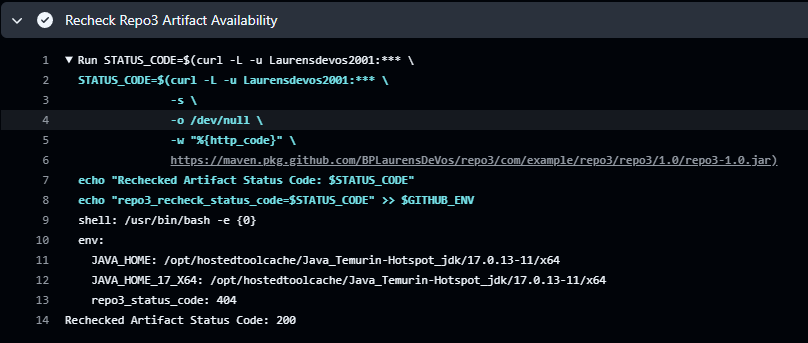
\includegraphics[width=\linewidth]{"C:/Users/laure/Documents/bachelorproef-2024-2025-laurensDeVos/graphics/mask.png"}
    \caption{Voorbeeld van logs in GitHub Actions waarin de gebruikersnaam zichtbaar is en tokens zijn gemaskeerd.}
    \label{fig:github_logs_actor}
\end{figure}

\paragraph{Vergelijking tussen Jenkins en GitHub Actions}
In de tabel \ref{tab:credentials_comparison} is een overzichtelijke vergelijking te zien tussen Jenkins en GitHub Actions.

\begin{table}[h!]
    \centering
    \begin{tabular}{|p{4cm}|p{5cm}|p{5cm}|}
        \hline
        \textbf{Aspect}               & \textbf{Jenkins}                                                                                                 & \textbf{GitHub Actions}                                                                                        \\ \hline
        \textbf{Beheer van credentials} & Credentials worden centraal beheerd in de Credential Store.                                                & Secrets worden beheerd op repositoryniveau via de instellingen van GitHub.                               \\ \hline
        \textbf{Bescherming in logboeken} & Credentials worden standaard gemaskeerd (\texttt{****}).                                                       & Secrets (\texttt{PAT\_TOKEN}) worden gemaskeerd, en gebruikersnamen kunnen optioneel worden gemaskeerd met extra configuratie. \\ \hline
        \textbf{Waarschuwingen}         & Geeft waarschuwingen voor onveilige praktijken zoals Groovy String interpolatie.                          & Geen waarschuwingen voor het gebruik van secrets in workflows, maar biedt een optie om gebruikersnamen te maskeren. \\ \hline
        \textbf{Flexibiliteit}          & Brede ondersteuning voor verschillende typen credentials (secret text, SSH-sleutels, certificaten, etc.). & Ondersteuning voor repository-, organisatie-, en omgevingsniveau secrets.                                                                 \\ \hline
    \end{tabular}
    \caption{Vergelijking van credentials management tussen Jenkins en GitHub Actions.}
    \label{tab:credentials_comparison}
\end{table}

\paragraph{Conclusie}

Jenkins biedt een robuust credentials management systeem met standaard masking en waarschuwingen voor onveilige praktijken. GitHub Actions biedt eenvoudiger integratie met GitHub, maar vereist extra configuratie om gebruikersnamen zoals \texttt{GITHUB\_ACTOR} te maskeren. Voor deze PoC is bewust gekozen om gebruikersnamen zichtbaar te laten in GitHub Actions, gezien het gebruik van dedicated CI/CD-accounts en de voordelen voor transparantie en debugging.

\subsubsection{Vergelijking op automatiseringsefficiëntie}

In deze sectie wordt de automatiseringsefficiëntie van Jenkins en GitHub Actions vergeleken. Hierbij wordt gekeken naar het configuratiegemak, het instellen van triggers en de algemene gebruikservaring.

\paragraph{Configuratiegemak}

De webinterfaces van zowel Jenkins als GitHub Actions bieden een gebruiksvriendelijke ervaring. Echter, er zijn enkele verschillen in het configuratieproces:
\begin{itemize}
    \item \textbf{Jenkins:} Het opzetten van een basispipeline in Jenkins vereist meer stappen. Gebruikers moeten eerst een pipeline-item aanmaken in de webinterface voordat ze kunnen beginnen met het schrijven van een Jenkinsfile. Daarnaast vereist Jenkins de installatie en configuratie van de tool zelf (in dit geval via Docker) en het installeren van aanvullende plug-ins, zoals Maven en SonarQube-integratie.
    
    \item \textbf{GitHub Actions:} In GitHub Actions kan direct een workflowbestand worden aangemaakt in de repository. Dit bespaart tijd omdat er geen extra configuratie in een aparte webinterface nodig is. Bovendien zijn er geen plug-ins die handmatig geïnstalleerd moeten worden, omdat GitHub Actions direct geïntegreerd is met GitHub en populaire acties zoals \texttt{actions/checkout} beschikbaar stelt.
\end{itemize}

Het schrijven van pipeline-code zelf verschilt ook tussen de tools:
\begin{itemize}
    \item \textbf{Jenkinsfiles:} Het schrijven van Jenkinsfiles wordt als intuïtiever ervaren vanwege de duidelijke en gestructureerde syntax. Dit maakt het eenvoudiger om complexe pipelines te configureren.
    \item \textbf{GitHub Actions files:} Hoewel GitHub Actions YAML-bestanden overzichtelijk zijn, kunnen ze complex worden wanneer meerdere afhankelijkheden en geavanceerde configuraties nodig zijn.
\end{itemize}

\paragraph{Triggers}

Het instellen van triggers voor pipeline- of workflowuitvoering toont belangrijke verschillen tussen de twee tools:
\begin{itemize}
    \item \textbf{Jenkins:} Jenkins biedt een intuïtieve manier om downstream jobs te configureren, waardoor pipelines automatisch worden getriggerd op basis van afhankelijke repositories. Deze functionaliteit is eenvoudig te configureren via de Jenkins-webinterface of direct in de Jenkinsfile.
    
    \item \textbf{GitHub Actions:} Het configureren van triggers met \texttt{repository\_dispatch} werkt beperkt, omdat de communicatie slechts in één richting plaatsvindt. Daarnaast is het noodzakelijk om een wachttijd (\texttt{sleep}) toe te voegen om te voorkomen dat downstream workflows falen vanwege ontbrekende artefacten. Dit maakt het beheer van afhankelijkheden complexer en minder efficiënt in GitHub Actions.
\end{itemize}

Afbeelding \ref{fig:jenkins_trigger} toont de configuratie van triggers in Jenkins, terwijl afbeelding \ref{fig:github_dispatch} een voorbeeld illustreert van het gebruik van \texttt{repository\_dispatch} in GitHub Actions.

\begin{figure}[h!]
    \centering
    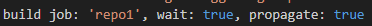
\includegraphics[width=\linewidth]{"C:/Users/laure/Documents/bachelorproef-2024-2025-laurensDeVos/graphics/jenkinstrigger.png"}
    \caption{Configuratie van downstream triggers in Jenkins.}
    \label{fig:jenkins_trigger}
\end{figure}

\begin{figure}[h!]
    \centering
    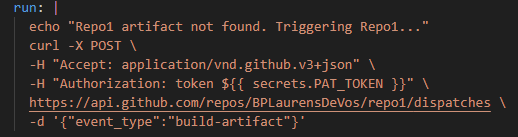
\includegraphics[width=\linewidth]{"C:/Users/laure/Documents/bachelorproef-2024-2025-laurensDeVos/graphics/actionstrigger.png"}
    \caption{Gebruik van \texttt{repository\_dispatch} in GitHub Actions.}
    \label{fig:github_dispatch}
\end{figure}

\paragraph{Conclusie}

Op het gebied van automatiseringsefficiëntie heeft GitHub Actions een voordeel in het snelle opzetten van eenvoudige workflows. Er is geen extra installatie of configuratie nodig, en workflows kunnen direct in GitHub worden beheerd. Voor meer complexe pipelines biedt Jenkins echter een robuustere oplossing, met betere ondersteuning voor triggers en afhankelijkheden tussen repositories. Dit maakt Jenkins geschikter voor scenario's met meerdere afhankelijkheden, zoals deze PoC.

\subsubsection{Integratie met bestaande systemen}
Dit onderdeel beoordeelt hoe goed Jenkins en GitHub Actions integreren met bestaande ontwikkelomgevingen en technologieën. Hierbij wordt specifiek gekeken naar de integratie met GitHub, Java, Maven en SonarCloud, zoals gebruikt in de Proof-of-Concept (PoC).

\paragraph{Integratie met GitHub}
\textbf{GitHub Actions} biedt een naadloze integratie met GitHub, aangezien het direct is ingebouwd in het platform. Workflows kunnen eenvoudig worden geactiveerd door gebeurtenissen zoals commits, pull requests of geplande taken. Dit maakt het opzetten van CI/CD-processen met GitHub Actions eenvoudig en intuïtief, zonder dat aanvullende configuraties nodig zijn.

In \textbf{Jenkins} vereist de integratie met GitHub meer configuratiestappen. De Git Plugin moet worden geïnstalleerd en geconfigureerd, waarna repositories handmatig moeten worden gekoppeld. Hoewel dit proces meer tijd kost, biedt het flexibiliteit door ondersteuning van meerdere versiebeheersystemen, niet beperkt tot GitHub.

\paragraph{Compatibiliteit met Java en Maven}
Beide tools bieden uitstekende ondersteuning voor Java en Maven. 
In de PoC zijn de volgende functionaliteiten geanalyseerd:
\begin{itemize}
    \item \textbf{GitHub Actions} gebruikt vooraf geconfigureerde acties uit de Marketplace, zoals \texttt{actions/setup-java}, voor het eenvoudig instellen van de juiste Java-versie en Maven-configuratie. Dit vereenvoudigt het proces aanzienlijk, met minimale handmatige configuratie.
    \item \textbf{Jenkins} maakt gebruik van de ingebouwde toolconfiguratie en plugins zoals de \texttt{Maven Integration Plugin}. Hoewel dit flexibiliteit biedt, vereist het meer handmatige configuratie, zoals het definiëren van tools en het instellen van specifieke versies.
\end{itemize}

\paragraph{Integratie met SonarCloud}
Voor kwaliteitscontrole en code-analyse is in de PoC SonarCloud geïntegreerd. 
\begin{itemize}
    \item In \textbf{GitHub Actions} is de integratie uitgevoerd met een officiële SonarCloud Action uit de Marketplace. Dit vereiste minimale configuratie en stelde de workflows in staat om naadloos analyses uit te voeren.
    \item In \textbf{Jenkins} werd de integratie bereikt door de installatie van de SonarQube Scanner Plugin. Dit proces vereist meer configuratiestappen, inclusief het handmatig instellen van de server-URL en authenticatietokens.
\end{itemize}

\paragraph{Conclusie}
GitHub Actions onderscheidt zich door zijn eenvoud en naadloze integratie met GitHub en andere ontwikkeltools, wat vooral voordelig is voor teams die volledig in het GitHub-ecosysteem werken. Jenkins biedt daarentegen meer flexibiliteit en kan beter worden aangepast aan complexe workflows of alternatieve versiebeheersystemen. Voor organisaties zoals DocShifter, die gebruik maken van Java en Maven, bieden beide tools voldoende ondersteuning. Echter, GitHub Actions kan worden aanbevolen voor snel op te zetten workflows, terwijl Jenkins geschikt is voor meer geavanceerde en op maat gemaakte integraties.

\begin{table}[h!]
    \centering
    \begin{tabular}{|p{5cm}|p{5cm}|p{5cm}|}
        \hline
        \textbf{Aspect} & \textbf{GitHub Actions} & \textbf{Jenkins} \\ \hline
        Integratie met GitHub & Naadloze ingebouwde integratie & Vereist handmatige configuratie met plugins \\ \hline
        Configuratie voor Java en Maven & Eenvoudig via Marketplace-acties & Flexibel, maar vereist meer handmatige configuratie \\ \hline
        Integratie met SonarCloud & Officiële actie beschikbaar in Marketplace & Vereist installatie en configuratie van plugins \\ \hline
    \end{tabular}
    \caption{Vergelijking van integratiekenmerken tussen GitHub Actions en Jenkins.}
    \label{tab:integration_comparison}
\end{table}


